\documentclass[thesis,appendsingle]{MSUstyle}
%
%  Created by Seth Humphries 
%  Update and maintained by Prof. Mark Owkes mark.owkes@montana.edu
% 
%%    Copyright (c) 2007-2012 Seth D. Humphries
%%    This work is licensed under the Creative Commons
%%    Attribution-Noncommercial-Share Alike 3.0 License. To view a copy
%%    of this license, visit http://creativecommons.org/licenses/by-nc-sa/3.0/;
%%    or, (b) send a letter to Creative Commons, 171 2nd Street, Suite
%%    300, San Francisco, California, 94105, USA. 
%
%  Version 2.0, check for periodic updates on the bitbucket repository
%
% DEFAULTS --------------------
% The default options are as follows:
%   \documentclass[12pt,letterpaper,oneside,openright,%
%       doublespaced,normalmargins,dissertation,final,numreset]{MSUstyle}
%
% default options do not need to be entered. Defaults will generate a document 
% that conforms to the MSU Electronic Thesis/Dissertation  (ETD) guidelines. 
%
% MASTERS THESIS ---------------
%  use \documentclass[thesis]{MSUstyle} to adjustment the front matter according to ETD style rules that
% are different for a thesis than for a dissertation.
%
% ADDITIONAL OPTIONS ----------
% 10pt, singlespaced, and draft allow you to require less number of pages for editing
% A draft version number can be set with, e.g., \draftver{1.0}
%
% altchapter provides numbered chapter and section titles
%
% appendsingle/appendmultiple is required if you have one/multiple appendices, remove if you do not have an appendix
%
% nonumreset does not add chapter to labels of figures, tables, etc. (not recommended)
%
% PRINTING OPTIONS ------------
% oneside,openright (defaults) larger margin on left side of pages (use for electronic documents and submission to grad school)
% twoside,openany  larger margins alternate left/right sides for binding (use for printing on minimal number of pages)
% twoside,openright larger margins alternate left/right sides for binding and ...
%                               blank pages added so chapter start on right page (use for nicest printed material)

% ========================= %
%         Packages  (add as needed)              %
% ========================= %
\usepackage[final]{graphicx} %for the \includegraphics command and figures put [final] before ...
%%    {graphix} if you want figures to show up even while in draft mode
\usepackage{subcaption}    % to be able to have multiple plots in one figure
\usepackage{color} % for changing text color in chapters \textcolor{red}{red text read here}. 
\usepackage{varioref}  % for \vref{figure} which shows up like ``figure 4 on page 6'' 
\usepackage[final]{listings} %used for formatting code
\usepackage[pdftex,hidelinks]{hyperref}
\usepackage{cite} %compresses the citations so \cite{ref1,ref2,ref3,ref4} is printed as [1-4] instead of [1,2,3,4]

\usepackage{amssymb}
\usepackage{amsmath}
\usepackage{xfrac}
\usepackage{caption}
\usepackage{xcolor}
\usepackage{graphicx}
\usepackage{float}
\usepackage{multicol}


% Math
\def\bm#1{\mbox{\boldmath{$#1$}}}


% Tikz
\usepackage{tikz}
\usetikzlibrary{calc}
\usetikzlibrary{patterns}
\usetikzlibrary{automata}
\usetikzlibrary{positioning}
\usetikzlibrary{decorations.markings}
\usetikzlibrary{decorations.pathmorphing,snakes}
\usetikzlibrary{fit}
\usetikzlibrary{intersections}
\usetikzlibrary{spy}
\usetikzlibrary{shadows.blur}
\usetikzlibrary{shapes.misc}
\usetikzlibrary{shapes.geometric}
\usetikzlibrary{fadings}
\usetikzlibrary{3d}
\usetikzlibrary{patterns}
\usepackage[most]{tcolorbox}
\usetikzlibrary{patterns}
\usetikzlibrary{arrows}
\usepackage[textsize=tiny]{todonotes}
\usepackage{soul}
\usepackage{fancyvrb}

\usepackage{amsmath}
\usepackage{enumitem}
\usepackage{lipsum} % Generates random text
\usepackage{color,soul} % Used for highlighting text -> only using while writing
%\usepackage{showframe} % View margins

% Style of code listings (Change as needed)
\lstset{%set Code listings styles
	language=Matlab, % program language for keywords and comments styles
	basicstyle=\small, %font size and style
	identifierstyle=\color{red}, %variable name style
	stringstyle=\ttfamily, %string style
	keywordstyle=\color{blue}\bfseries, %language keyword style
	commentstyle=\color{black}\itshape, %commentstyle
	breaklines=true,  % sets automatic line breaking
	breakatwhitespace=false,   %break line not just at whitespaces
}


% ======================= %
%  User defined commands (  %
% ======================= %
\newcommand{\etc}{etc.}
\newcommand{\eg}{e.g.}
\newcommand{\ie}{i.e.} 

% ======================= %
%       User defined clolors          %
% ======================= %
\definecolor{lightblue}{HTML}{9ACCCD}

% =============================== %
%  Definitions: Change as needed  %
% =============================== %
\name{Kristopher Thomas Olshefski} %PUT your FULL name here (First Middle Last)
\DocTitle{Conservative Simulations of Atomization\\ Applying the Height Function Method to Rudman Dual Grids } 
\OWNwebpage{http://mywebsite.net} %your personal webpage
\degreetitle{Mechanical Engineering} % may be different than department... ie MS in Electrical Engineering is not Elect. and Com. Engnr degree.
\department{Mechanical \& Industrial Engineering} 
\committeechair{Dr. Kevin S. Repasky} 
\departmentchair{Dr. Robert C. Maher}
\graduatedean{Dr. Carl A. Fox}
\submitdate{November 2019} 
\copyrightyear{2019} % add one to year if document submitted in Dec.
%\draftver{1.0} % versioning for use with draft option

% put searchable words you want internet search engines to find here
\keys{Engineering, Thesis, Template, Latex, Montana, Montana State University} 
 
%\bibfiles{mybib} %your .bib file(s), files containing bibliographic 

%  Configuration of hyperref package
\hypersetup{%
	baseurl={\OWNwebpage}, %baseurl is url that is in pdf document properties
% 	bookmarks=true, %show bookmarks when opening pdf
	citecolor=black, %citations show up black
	colorlinks=true, %use colored links
	draft=false, % prevents hyperref from draft mode...keeps bookmarks and hyperlinks in draft mode
	filecolor=black, %included file links are black text
	linkcolor=black, %the colored links are black for an ETD but can be otherwise
	pdfauthor={\name}, %pdf document maker is you
	pdfcreator={\name \ by \ PDFLaTex}, %pdf document maker is you
	pdfdisplaydoctitle=true, % make display title the same as the document title instead of the filename
	pdffitwindow=true, %fits one page into the open pdf reader window
	pdfkeywords={\keys}, %searchable keywords
	pdfsubject={\degreetype \ for \name}, %the \  is to give a space
	pdftitle={\DocTitle}, %pdf document title is now ETD title
	plainpages=false, %use hyperlinks in pages, gets rid of a lot of warnings too
	urlcolor=black %website links are black text
}%

% ================================ %
%         Actual Document                                              %
% ================================ %
\begin{document}

% Front matter...before your text
\begin{preliminary} 

  % Dedication page (optional, comment out if not using)
%  \begin{dedication} 
%    % Dedication

I dedicate this to all MSU students who use \LaTeX.  Dedication is optional and may be no longer than one page, single spaced, and should precede the acknowledgments page.  


 
%  \end{dedication}
%
%  % Acknowledgements page (optional, comment out if not using)
%  \begin{acknowledgements}
%    % Acknowledgement

I would like acknowledge\dots Acknowledgments must be double spaced and is limited to one page. Consider that you may need to include a funding acknowledgement.

 
%  \end{acknowledgements}
%
%  %vita page (optional, comment out if not using)
%  \begin{vita}
%    % Vita

Chris Jordan Doe was born in Bozeman, MT in 1893.  Raised by Champ, Chris is a true Bobcat. Chris attended Bozeman High and graduated with honors. After high school, \dots

If you include a vita, it should contain the full name of the author, date and place of birth, parentage, secondary education, and collegiate degrees. The vita should be written in essay form in the third person and may not exceed one single-spaced page.

 
%  \end{vita}

  % Table of Contents, List of Figures|Tables|etc.
  \contents

  % Nomenclature page (optional, comment out if not using)
  \begin{nomen}
    % Nomenclature 

\begin{tabular}{l l}
  $\mu$ & Dynamic viscosity \\
  $\mathbf{n}$ & Normal vector\\
  $\mathbf{u}$ & Velocity vector
\end{tabular}
 
  \end{nomen}

  % Abstract
  \begin{abstract}
    % Abstract 
%The abstract must be single spaced and no more than 350 words. The abstract must contain the following elements: (1) statement of the problem, (2) procedure or methods, (3) results, and (4) conclusions. Mathematical formulas, abbreviations, diagrams, and other illustrative materials should not be included. It should be written to be understood by a person who does not have expertise in the field.

Gas-liquid flows can be significantly influenced by the surface tension force, which controls the shape of the interface. The surface tension force is directly proportional to the interface curvature and an accurate calculation of curvature is essential for predictive simulations of the flow types. Furthermore, methods that consistently and conservatively transport momentum, which is discontinuous at the gas-liquid interface, are necessary for robust and accurate simulations. Using a Rudman dual mesh, which discretizes density on a twice as fine mesh, provides consistent and conservative discretizations of mass and momentum. The height function method is a common technique to compute an accurate curvature as it is straightforward to implement and provides a second-order calculation. 

When a dual grid is used, the standard height function method fails to capture fine grid interface perturbations and these perturbations can grow. When these growing perturbations are left uncorrected, they can result in nonphysical dynamics and eventual simulation failure. This work extends the standard height function method to include information from the Rudman dual mesh. The proposed method leverages a fine-grid height function method to compute the fine-gird interface perturbations and uses a fine-grid velocity field to oppose the fine-grid perturbations. This approach maintains consistent mass and momentum transport while also providing accurate interface transport that avoids non-physical dynamics. The method is tested using an oscillating droplet test case and compared to a standard height function. Various iterations of the fine grid method are presented and strengths and shortcomings of each are discussed. 
  \end{abstract}
\end{preliminary}

% Dissertation chapters:  add/change as needed
\chapter{Introduction}\label{CH:introduction}

%******* WHY DONT YOU START INTRODUCING SURFACE TENSION HERE? TALK ABOUT ITS IMPORTANCE FOR ACUURATELY MODELING FLOWS*******

The study of fluid dynamics covers a wide array of phenomena across large spans of scales. Current research can be found exploring everything from biomedical simulations of capillary flows~\cite{1} to astrophysical approximations of star formations~\cite{1}. Researchers are studying bio-inspired dynamics of animals to gain insight into efficiency shortcomings of man made vessels~\cite{1}. Other research focuses on oceanic current modeling to gain a deeper understanding of the natural world~\cite{1}. The focus of this research however, is on multiphase flows. In the context of this research, interest is restricted to flows where both a liquid and gas are present. These flows are referred to as gas-liquid flows, multiphase flows, or free surface flows in literature~\cite{1,2,3}. Examples of gas-liquid flows can be seen throughout the natural world as well as industrial application and may be some of the most wide spread and common flow types on Earth. Bubbles rising in a carbonated drink, rain falling through the air, paint exiting a can of spray paint, a wave on the surface of the ocean; these are all examples of gas-liquid multiphase flows. These types of flows are of particular academic interest due to the ubiquity with which they emerge in industrial and engineering applications. For example, the increasing efficiency of internal combustion engines over the past several decades can \hl{largely be attributed}\todo{need a reference for a statement like this} to an increased understanding of the physics at work during fuel combustion. For efficient combustion to occur in a gasoline engine the fuel must first be atomized. Atomization is the process by which the fuel is broken from a stream into a fine mist or distribution of smaller droplets.


For engineering applications there are two main pathways by which multiphase flows are studied. Experimentation is a common method of study inside many scientific disciplines; the field of fluid dynamics is no different. Many researchers design experimental studies to gain deeper insight into the behavior of multiphase flows. Some examples of experimental techniques include shadowgraphy, x-ray imaging, or Particle image velocimetry (PIV) \todo{Include references for these techniques or reference a review paper}. Computational fluid dynamics (CFD) is the second avenue used in multiphase flow study and is the focus this research.  CFD employs the computational power of modern computing to digitally investigate fluid flow problems. 


Within the field of CFD, simulation models are often classified by the scale to which they resolve turbulent structures. However, these methods all share the commonality that in some form or another, they all solve the Navier-Stokes equations which govern fluid flow. While many approaches exist, there are three main schemes: Reynolds Averaged Navier-Stokes (RANS), Large Eddy Simulation (LES), and Direct Numerical Simulation (DNS). These methods scale in fidelity respectively. RANS methods solve the time averaged Navier-Stokes equations. This is the least computationally intense method of the three but requires a modeling scheme for all turbulent structures. Due to its low computational cost, RANS models are most commonly seen in industry application where a rough approximation of the turbulence scale is sufficient for design purposes. LES models are more computationally expensive than RANS models but are still fairly common in industrial engineering applications as well as academic research. LES methods solve filtered Navier-Stokes equations. This means that a filter is applied to the governing equations and then a closure model allows for the numerical simulation of the equations. The filtering operation and subsequent closure models give LES methods the ability to resolve some larger turbulent structures within a flow. While DNS methods are the most expensive of the three, they have the advantage of providing the most complete solution of the mathematical model. This is because direct simulations resolve the entire range of turbulent scales with no modeling necessary. Due to the computational expense however, DNS methods are usually reserved for academic interests in which a critical understanding of the realistic flow characteristics is required. An example of a simulated atomizing jet can be seen in Figure \ref{fig:DNSjet}. The image in this figure was produced from a DNS simulation. DNS methodology is the focus of this research.
\todo[inline]{It would be useful to have a paragraph on how gas-liquid flows can be modeled with RANS, LES, or DNS.  With RANS, break-up models are used (see Clarks' paper for a list of references), there some work on LES but there are challenges (see work of Herrmann and Wojciech (Wojtek) ANISZEWSKI.)}

\begin{figure}[htbp]
	\centering
	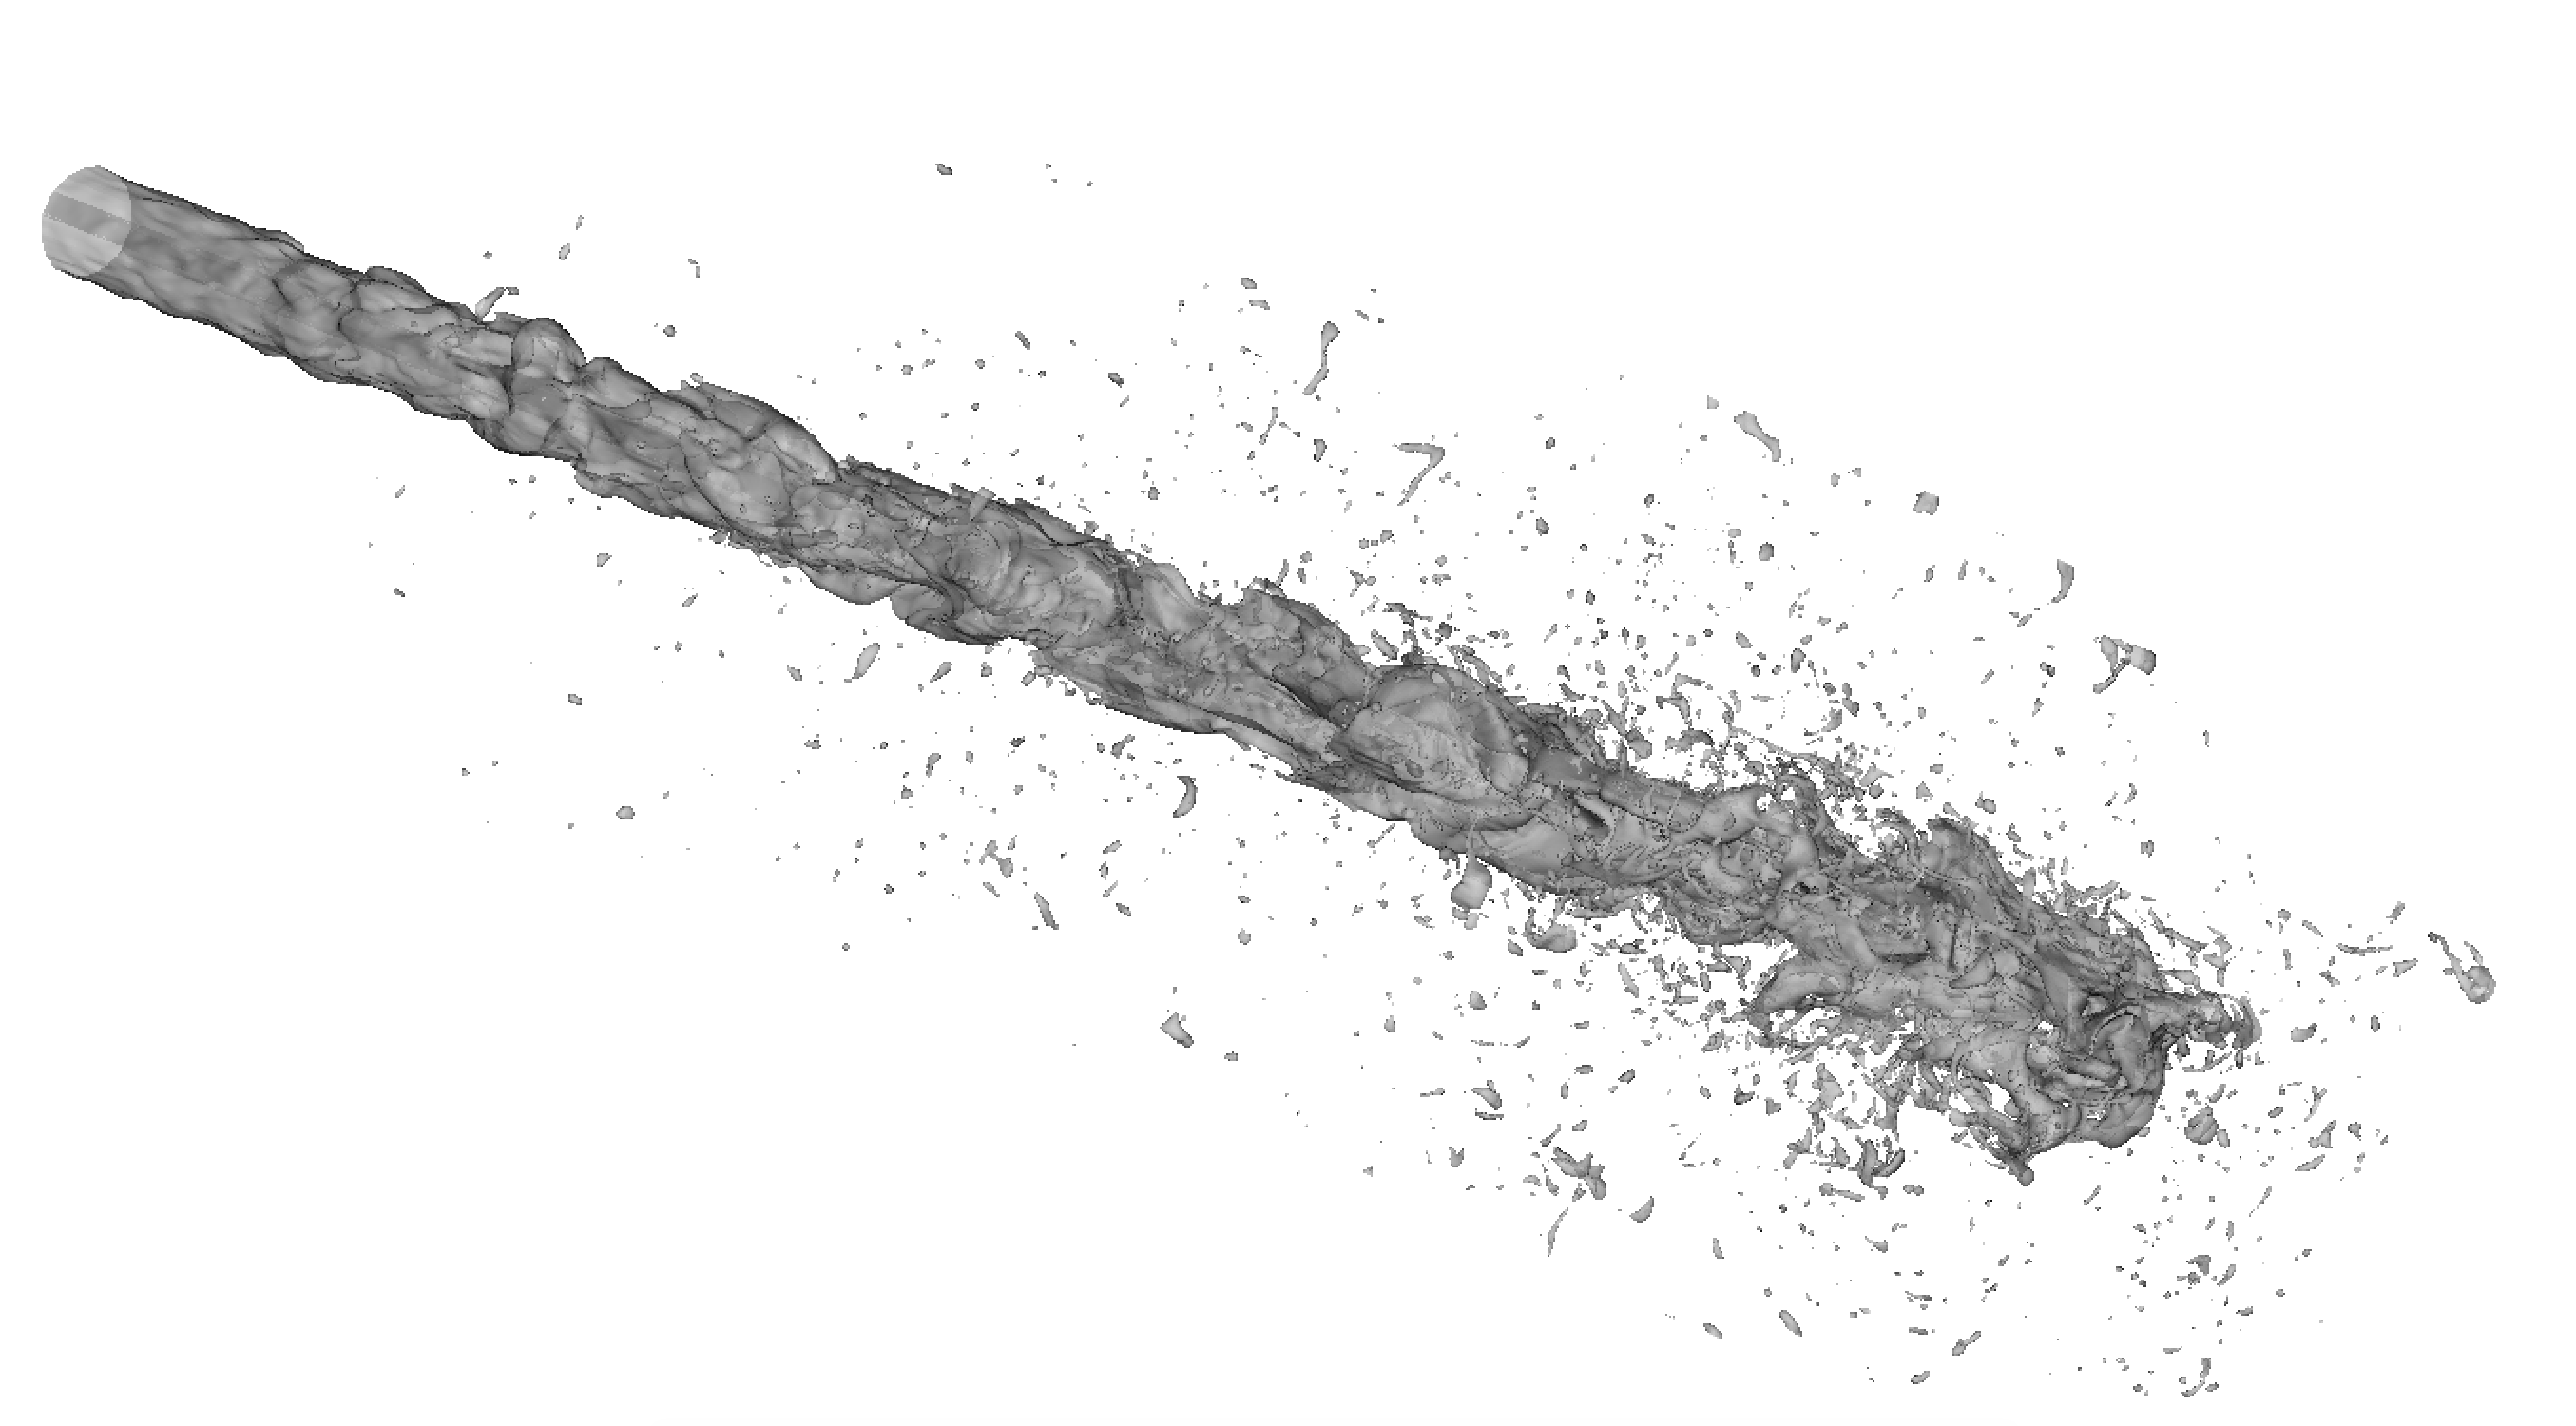
\includegraphics[width=0.8\textwidth]{figs/ACESjet}
	\caption{DNS Simulation of Atomizing Jet}
	\label{fig:DNSjet}
\end{figure}

Those involved in research using CFD can be segregated into \hl{two groups}\todo{unclear what the two groups are in this paragraph} based on their research focus. Simulation based research utilizes in-house or commercial software packages to answer specific questions about fluid flow. An example of this might be a researcher trying to optimize an airfoil shape for specific flight conditions. With any number of software packages, various shapes and flow conditions can be simulated to determine an optimal geometry. Numerical methods for fluid dynamics focus on the accurate and efficient implementation of the Navier-Stokes equations, the governing equations of fluid mechanics, into numerical algorithms. An example of this might be the development of a new, more computationally efficient, method for solving partial differential equations. The focus of the research presented in this paper falls into this category.
\todo[inline]{It would be useful to give some examples of industrial applications as well as some recent algorithm development}.

Numerous challenges exist concerning numerical methods of multiphase flows. One challenge of particular interest is the accurate representation of the \hl{intersection}\todo{I would just call this an interface and skip the intersection step.} of the two fluids which exists for all gas-liquid multiphase flows. This intersection, known as the gas-liquid interface, presents notable challenge because the transition from one phase to another is represented as a mathematical \hl{discontinuity}\todo{somethings are continuous and other's are not}. That is, the change in density of the two fluids at the interface, is decidedly difficult to approximate mathematically. Surface tension is the governing force controlling the shape and behavior of the interface. For constant surface tension coefficient \todo{what changes if $\sigma$ is not constant?}, the surface force ($\textbf{f}_{\sigma}$) is expressed as $\textbf{f}_{\sigma} = \sigma \kappa \textbf{n}$\cite{desjardins_direct_2013}. Here, $\sigma$ is given as the surface tension coefficient, a value empirically determined forfluids. The vector perpendicular to the interface is \textbf{n}. The curvature of the interface is given by $\kappa$. Various curvature estimation schemes exist. Review of the mechanics which are required for this estimation along with a novel curvature scheme are the focus of the research to be discussed in the remainder of this work.
\todo[inline]{A paragraph (or two) focused on why the surface tension force is important, it's effect of fluid, where it comes from etc. would be interesting.}

 
%Stuff taken from past paper

%	Numerical models of surface tension play an important role in accurately predicting the behavior of multiphase flows such as those seen in the atomization process. Interface curvature is directly proportional to the surface tension force and controls many of the dynamics of an atomizing jet. Therefore, an accurate curvature calculation is vital for realistic analysis.  Height function methods (HFM) are a popular way of computing interface curvature in volume-of-fluid (VoF) architectures and were first introduced in the context of two-phase flows by Sussman~\cite{Sussman2003}. Standard height function methods, as seen in Fig.~\ref{fig:HFM}, calculate interfacial curvature by applying finite difference operators to heights which neighbor a cell of interest.


%\begin{figure}[h]

%	\begin{center}

%		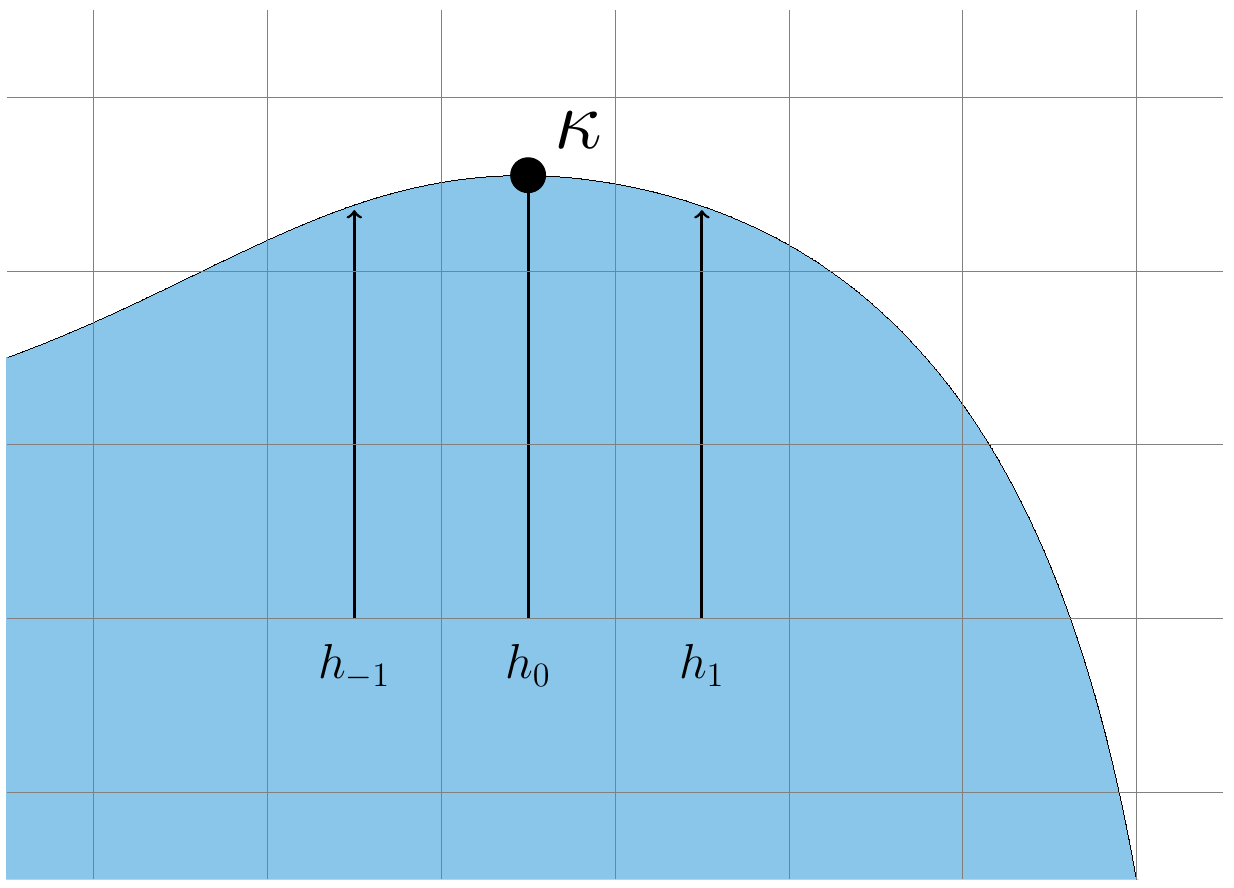
\includegraphics[width=2.5in]{figs/HFM.png}

%	\end{center}

%	\caption{Standard height function.}

%	\label{fig:HFM}

%\end{figure}


%Traditional mesh configurations calculate density at cell centers and momentum at cell faces. This can allow for an uncoupling of mass and momentum advection. Using a Rudman dual grid, which discretizes density on a twice as fine mesh, provides consistent and conservative discretizations by calculating fluxes on sub-faces~\cite{Rudman1998}. However when a dual grid is used, the standard height function method fails to capture fine grid interface perturbations. 	These perturbations can grow uncontrollably and result in non-physical dynamics occurring in simulations. An example of tihs uncontrolled growth resulting in non-physical dynamics can be seen in Fig.~\ref{bad2}. This research develops an extension of the standard height function to include information from the Rudman dual mesh. This method results in consistent mass and momentum transport while also providing accurate interface transport that avoids non-physical dynamics.



\chapter{Theory} \label{CH:theory}
%\textbf{What is your thought process in how to solve this problem??\\
%How do you propose solving this problem?\\
%What is a dual grid?\\
%What is a height function?\\
%How does it work?\\
%Why do we choose to use a HFM?\\
%Shortcomings of HFM's?\\
%On this dual grid, why do we need a fine velocity?}\\
\hl{Computational solutions for fluid flow rely on several fundamental ideas surrounding how fluids are simulated.}\todo{Not sure what this says} The following section is an attempt to summarize several of these methods and lay the necessary framework for understanding the subsequent method, which is the primary focus of this work. Each of the methods discussed are present within NGA, the computational platform used in this research. Additionally, while these methods are prevalent in the CFD community, they are not the only options available. The interested reader is directed to \ref{TRYG} for a more comprehensive assessment.   

\subsection{The Navier-Stokes Equations}
They exist, here they are....
\hl{consider discussion}

\subsection{Computational Platform}
\todo{This section sounds ``very'' familiar, should probably paraphrase into your own words (read it, take notes, and then write it.} The proposed curvature estimation method exists as a module within a larger computational framework. While this scheme can be incorporated into any number of solvers, the platform used for this work was NGA~\cite{NGA1,NGA2}.  NGA solves low-Mach number, variable density formulations of mass and momentum conservation laws
\begin{align}
\frac{\partial \rho_\phi}{\partial t} +& \nabla \cdot \left(\rho_\phi\bm{u}_\phi\right) = 0\mbox{ \quad and}\\
\frac{\partial \rho_\phi \bm{u}_\phi}{\partial t} +& \nabla \cdot \left(\rho_\phi\bm{u}_\phi\otimes\bm{u}_\phi\right) = -\nabla p_\phi + \nabla\cdot\left(\mu_\phi\left[\nabla\bm{u}_\phi+\nabla\bm{u}_\phi^\mathsf{T}\right]\right)+\rho_\phi\bm{g}
\end{align}
where
$\rho_\phi$ is the density,
$\bm{u}_\phi=[u,v,w]_\phi$ is the velocity field vector,
$t$ is time,
$p_\phi$ is the hydrodynamic pressure,
$\mu_\phi$ is the dynamic viscosity, and
$\bm{g}$ is the gravitational acceleration.
The subscript
$\phi$ indicates the phase and takes values of $\phi=g$ or
$\phi=l$ in the gas or liquid phase, respectively.

These equations have been written in both the gas and liquid phases and are connected through jump conditions at the phase interface.
For example, the jumps in density and viscosity at the interface
$\Gamma$ are written as 
\begin{align}
[\rho]_\Gamma&%
=\rho_l-\rho_g\mbox{\quad and}\\
[\mu]_\Gamma&%
=\mu_l-\mu_g.
\end{align}
In the absence of a phase change, the velocity field is continuous, \ie,
\begin{equation}
[\bm{u}]_\Gamma=0.
\end{equation}
The pressure is discontinuous due to contributions from surface tension and the normal component of the viscous stress, \ie,
\begin{equation}
[p]_\Gamma=\sigma\kappa+ 2\left[\mu\right]_\Gamma\bm{n}^\mathsf{T}\cdot\nabla\bm{u}\cdot\bm{n},
\end{equation}
where
$\sigma$ is the surface tension coefficient and
$\kappa$ is the interface curvature. This is the curvature that is computed with the height function method.

These equations are discretized using a Cartesian mesh with pressure and other scalars located at cell centers and velocity components located at cell faces. Time is discretized using an iterative second order Crank-Nicolson formulation with a semi-implicit correction on each subiteration~\cite{choi}. The interface is represented with a geometric volume-of-fluid (VoF) method~\cite{Owkes2017,Owkes2014}. The NGA code is highly parallelized, allowing for scalable simulations and fast run times and has been applied to many atomization applications~\cite{OwkesAIAA,Desjardins2013,sheehy}.

\subsection{Mesh Generation}
In Numerical analysis, the grid or mesh, often refers to the manner in which a domain being simulated is subdivided into smaller sections and points. Traditionally these points are denoted using an i,j scheme and neighboring points will be referenced from an initial point as seen in Figure \ref{fig:ijGrid}. This method is extended similarly in the z-direction for 3D applications~\cite{MIT}.  

	\begin{figure}[htbp]
		\centering
		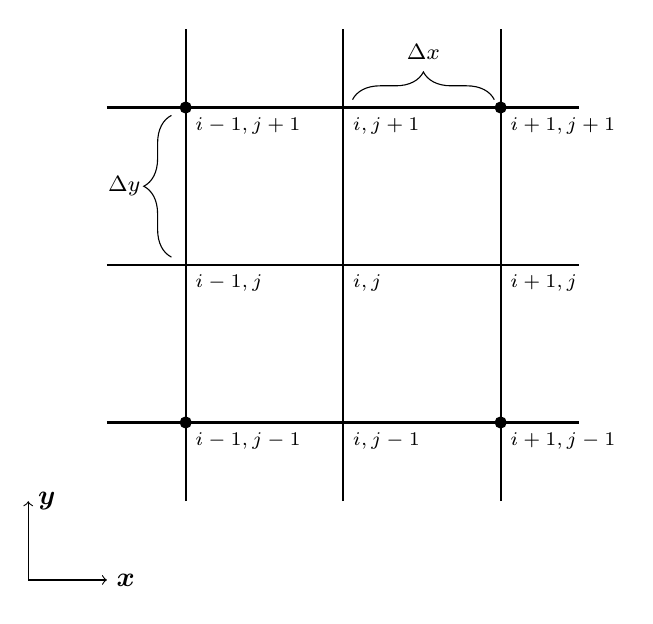
\begin{tikzpicture}[scale=2.0]
		% Mesh
		\draw [black,thick,step=1.0] (0.5 , 0.5) grid (3.5,3.5); 
		% i's and j's
			\node[below right] at (1,1) {\scriptsize{$i-1,j-1$}};
			\node[below right] at (1,2) {\scriptsize{$i-1,j$}};
			\node[below right] at (1,3) {\scriptsize{$i-1,j+1$}};
			\node[below right] at (2,1) {\scriptsize{$i,j-1$}};
			\node[below right] at (2,2) {\scriptsize{$i,j$}};
			\node[below right] at (2,3) {\scriptsize{$i,j+1$}};
			\node[below right] at (3,1) {\scriptsize{$i+1,j-1$}};
			\node[below right] at (3,2) {\scriptsize{$i+1,j$}};
			\node[below right] at (3,3) {\scriptsize{$i+1,j+1$}};
		%Node Circles
			% \draw [fill] (2,2) circle [radius=0.035];
			% \draw [fill] (1,2) circle [radius=0.035];
			% \draw [fill] (3,2) circle [radius=0.035];
			% \draw [fill] (2,1) circle [radius=0.035];
			% \draw [fill] (2,3) circle [radius=0.035];	
			% \draw [fill] (1,1) circle [radius=0.035];
			% \draw [fill] (1,3) circle [radius=0.035];
			% \draw [fill] (3,1) circle [radius=0.035];
			% \draw [fill] (3,3) circle [radius=0.035];
                        \foreach \x in {1,3} {
                          \foreach \y in {1,3} {
                            \draw [fill] (\x,\y) circle [radius=0.035];
                          }
                        }
                        
                        
		%Axes
			\draw [arrows=->] (0,0) -- node[pos=1,right] {$\bm{x}$} (0.5,0);
			\draw [arrows=->] (0,0) -- node[pos=1,right] {$\bm{y}$} (0,0.5);
		%Dx Dy
			\draw [decorate,decoration={brace,amplitude=10pt},xshift=-4pt,yshift=0pt] (1.05,2.05) -- (1.05,2.95) node [black,midway,xshift=-0.6cm] {\footnotesize $\Delta y$};
			\draw [decorate,decoration={brace,amplitude=10pt},xshift=-4pt,yshift=0pt] (2.2,3.05) -- (3.1,3.05) node [black,midway,yshift=0.6cm] {\footnotesize $\Delta x$};
		\end{tikzpicture}
		\caption{Typical notation of structured grid cells. }
		\label{fig:ijGrid}
	\end{figure}\todo{try foreach loop! this would be more informative if you showed the staggered grid with the location of $P$, $u$, $v$, $VOF=\alpha$.}

\paragraph{} The type of grid used can be classified as being in one of two categories, structured or unstructured~\cite{anderson}. The choice of whether to use a structured or unstructured grid should be considered on a case by case basis. However, there are some important characteristics of each that are important to recognize prior to implementation. A structured grid in 2D can be thought of a series of quadrilateral elements (bricks) placed side by side in a uniform fashion~\cite{MIT}. Here, neighboring elements are referenced by adding or subtracting from the base cell indices~\cite{anderson}. Figure \ref{fig:Simple Grid} is an example of a structured grid. An unstructured grid does not retain uniformity and is \hl{normally (although, not always)}\todo{really?} comprised of triangular elements~\cite{tu}. To reference neighboring cells in an unstructured grid, storage of cell-to-cell pointers are required~\cite{MIT}. Unstructured grids normally require a greater amount of memory storage and can result in slower computation times than that of a structured grid~\cite{magoules}. A simplified example of an unstructured grid can be referenced in Figure \ref{fig:Unstructured Grid}. The NGA code, which is this focus of this research, uses a structured grid approach for simplicity and computational efficiency. However, it should be noted that unstructured grids are increasing in popularity as the accuracy obtained from modeling complex flow geometry may be higher than that of a structured grid~\cite{Hirt1981}. 

\begin{figure}[htbp]
	\centering
	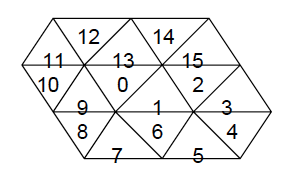
\includegraphics[width=2.5in]{figs/unstruc}
	\caption{Simple Unstructured Grid \cite{MIT}}
	\label{fig:Unstructured Grid}
\end{figure}

\subsection{Volume of Fluid Formulation}\todo{Should have a broader section on interface tracking and capturing schemes and explain why VOF is often used.}
In order to accurately predict the behavior of a multiphase system, the location of the interface of the two fluids must be determined. One method for completing this is known as the Volume of Fluid (VOF) method \todo{give mathematical definition of volume of fluid}. This method was first introduced by Hirt \& Nichols (1981) and has been expanded upon by several others~\cite{Hirt1981,1,2,3,4}. The defining contribution of the VOF method proposed by Hirt \& Nichols is the introduction of a scalar marker function assigned to each mesh cell which is indicative of the volume of a given fluid within that cell~\cite{Hirt1981}. This allows for interface to be tracked by the value of the marker cell in surrounding cells. For example, if $VOF = 1.0$ indicates a region of liquid and $VOF = 0.0$ indicates a region of gas, then a cell with a value $0.0 \leq VOF \leq 1.0$ indicates a cell which contains interface. It is important to recognize that volume of a fluid may only be advected into a new cell once the current cell is full~\cite{TRYG} \todo{this is true for 1D problems but not in general}. A one-dimensional example of this advection can be seen in Figure \ref{fig:1Dadvect}.

\begin{figure}[htbp]
	\centering
	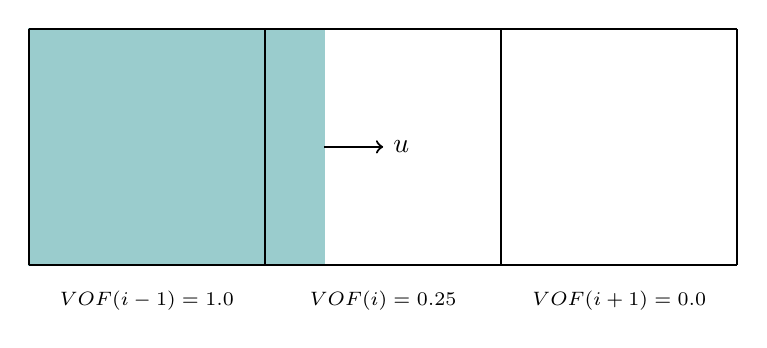
\begin{tikzpicture}[scale=3.0]
	% Mesh
	\draw [lightblue,fill=lightblue] (0.0,0.0) -- (1.25,0.0) -- (1.25,1.0) -- (0.0,1.0) -- cycle;
	\draw [black,thick,step=1.0] (0.0 , 0.0) grid (3.0,1.0); 
	%Velocity
	\draw [arrows=->, thick] (1.25,0.5) -- node[pos=1,right] {$u$} (1.5,0.5);
	%Labels
	\node[] at (0.5,-0.15) {\scriptsize{$VOF(i-1)=1.0$}};
	\node[] at (1.5,-0.15) {\scriptsize{$VOF(i)=0.25$}};
	\node[] at (2.5,-0.15) {\scriptsize{$VOF(i+1)=0.0$}};
	\end{tikzpicture}
	\caption{Advection of a one-dimensional fluid interface}
	\label{fig:1Dadvect}
\end{figure}

The advection procedure for a VOF method is completed in two primary steps. First, the interface needs to be geometrically constructed. Second, the constructed interface is advected with the current velocity field\cite{TRYG}. Figure \ref{fig:1Dadvect} depicts one-dimensional interface advection. In this case, geometric reconstruction is accomplished with a single vertical line. Adoption of this method is straightforward. As simulations increase to two or three dimensional analysis however, this problem quickly becomes non-trivial. Early attempts to resolve this difficulty include the Simple Line Interface Calculation (SLIC) method of Noh and Woodward (1976)\cite{NohWoodward}. Here, the reconstructed interface is made up of lines which align parallel to the mesh in both \textit{x} and \textit{y} directions.      
     
\begin{figure}[htbp]
	\centering
	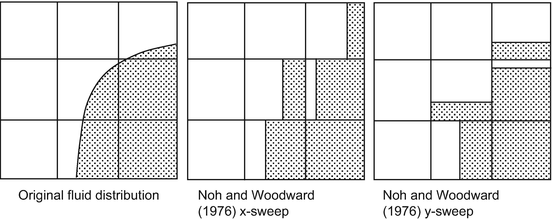
\includegraphics[width=0.7\textwidth]{figs/SLIC.png}
	\caption{Simple Line Interface Calculation of Noh and Woodward adapted from \cite{SLICfig}}
	\label{fig:SLIC}
\end{figure}

Improvement to the SLIC method was presented by Youngs (1982)  known as the Piecewise Linear Interface Calculation (PLIC)~\cite{youngs}. In the PLIC method, instead of aligning interfacial reconstruction lines with the mesh, a line (2D) or plane (3D) is oriented with a normal vector which is evaluated from the volume fraction gradient~\cite{yeoh}. An example of PLIC can be seen in Figure \ref{fig:PLIC}. This method is a popular geometric reconstruction scheme still today and is used in NGA for this research.

\begin{figure}[htbp]
	\centering
	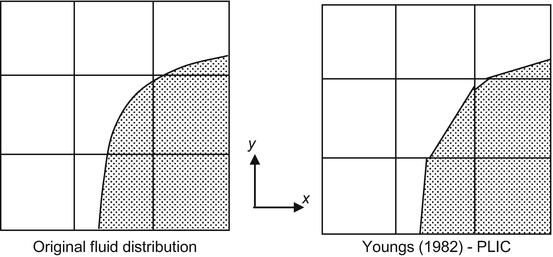
\includegraphics[width=0.5\textwidth]{figs/PLIC.png}
	\caption{Piecewise Linear Interface Calculation of Youngs adapted from \cite{yeoh}}
	\label{fig:PLIC}
\end{figure}

\todo{should mention other options such as PROST}
\subsection{Rudman Dual Grid Formulation}
Solution of the incompressible Navier-Stokes equations traditionally occurs on whats known as a staggered grid. On a staggered grid, pressure is typically stored at cell centers and velocity components are stored at cell faces~\cite{TRYG}. Building from the structured grid example given in Figure \ref{fig:ijGrid}, this implementation is illustrated in Figure \ref{fig:StagGrid}. 

 \begin{figure}[h!]
 	\centering
 	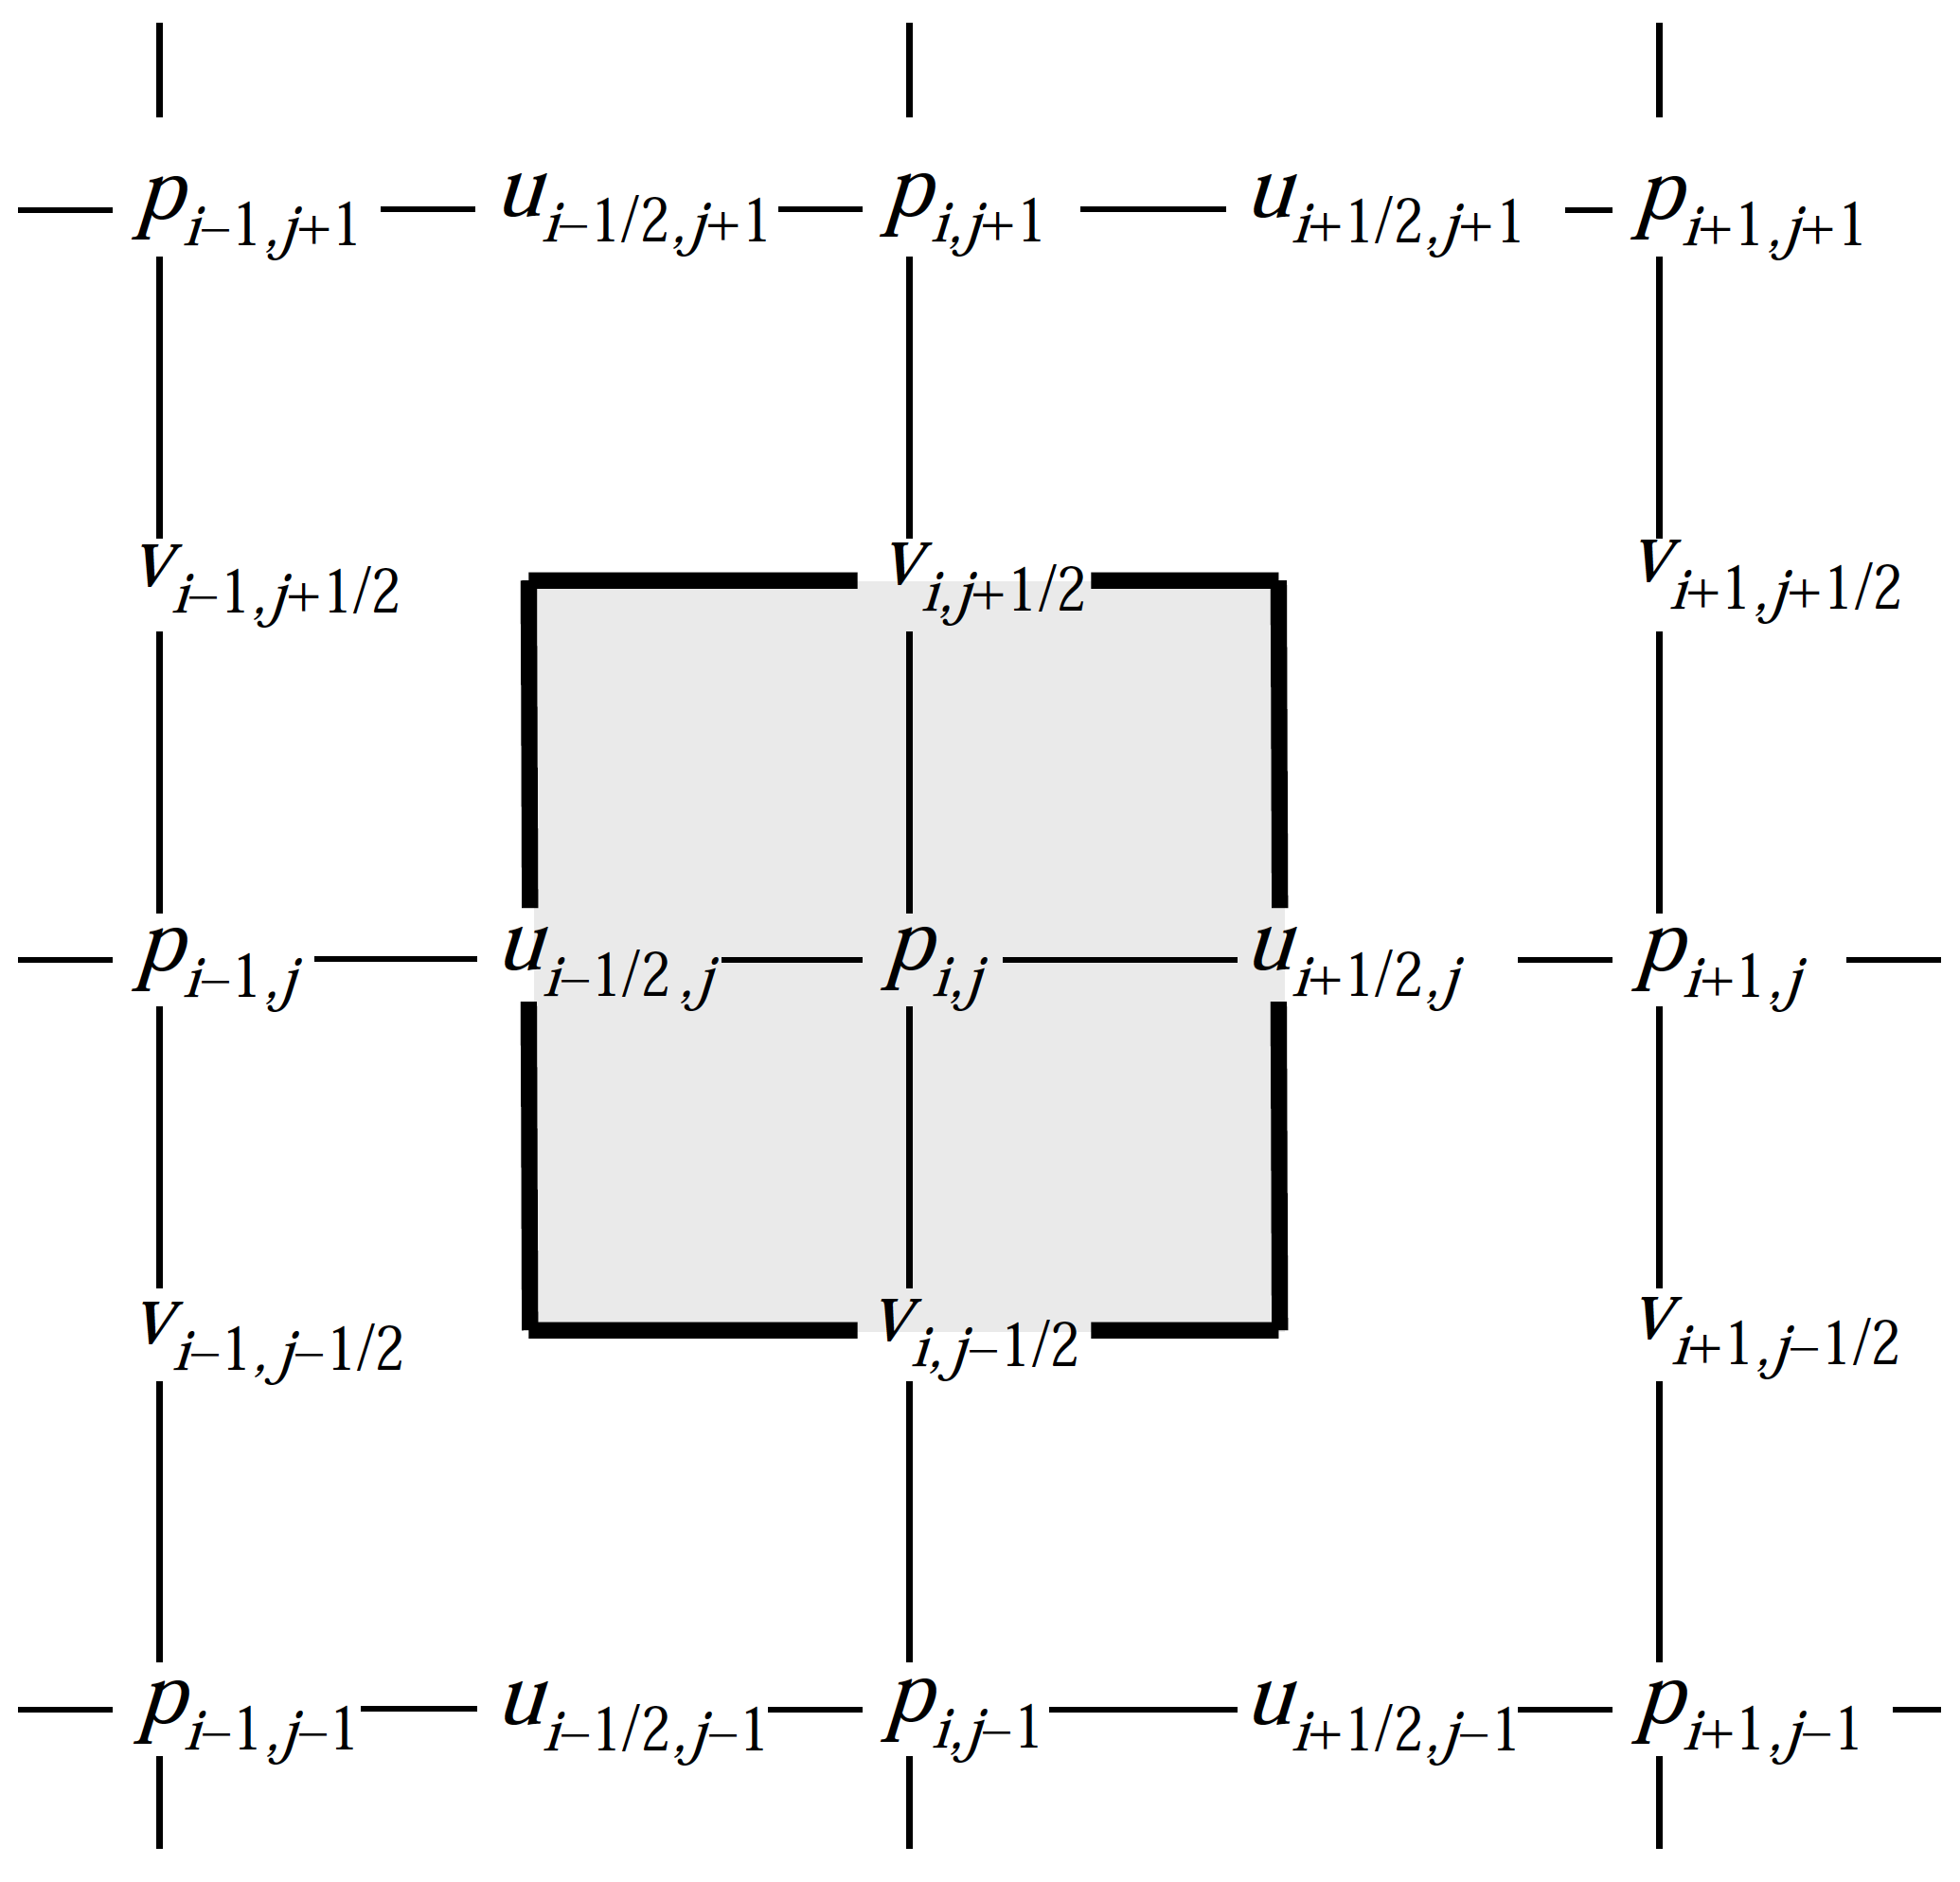
\includegraphics[width=2.5in]{figs/StaggeredGrid}
 	\caption{Typical staggered grid, adopted from \cite{TRYG}.}
 	\label{fig:StagGrid}
 \end{figure}

\todo{why no indent? if you want to put a figure call inside a paragraph, that is fine, just don't put empty lines before or after the figure.}\noindent This approach was first introduced by Harlow and Welch (1965) and is now considered the standard approach in structured mesh CFD applications today \cite{HARLOW1965}. For incompressible flows, staggered grids offer the advantage of tightly coupling fluid property variables as well as eliminating pressure-velocity checkerboarding~\cite{rudman}. The Rudman Dual grid approach, first presented by Rudman (1998), is a technique developed for high density ratio, multiphase flows, which accurately conserves both mass and momentum. This is achieved by calculating momentum-flux values on a twice as fine mesh near the fluid interface as illustrated in Figure \ref{fig:rudmesh}~\cite{Rudman}. The Rudman Dual mesh is incorporated into NGA and is essential to the formulation of the method presented in this research. \todo{Need more here.  how does a dual grid provide conservation. do other options exist?}

\begin{figure}[htbp]
	\centering
	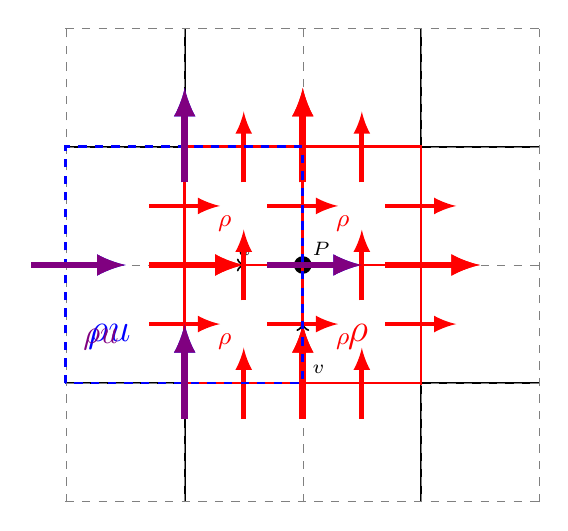
\begin{tikzpicture}[scale=3]
	% Mesh
	\draw [black,thick,step=1.0] (1.5 , 1.5) grid (3.5,3.5);
	\draw [dashed,step=0.5, help lines] (1.495 ,1.495) grid (3.5,3.5);
	%Cell centered dots
	\draw [fill] (2.5,2.5) circle [radius=0.035];
		% Pressure nodes
		\node [above right] at (2.5,2.5) {\scriptsize{$P$}};
%	% U Velocity Arrows
	\draw [arrows=->,line width=0.75] (2.0,2.5) -- (2.25,2.5);

		\node [above] at (2.25,2.5) {\scriptsize{$u$}};
		\draw [arrows=->,line width=0.75] (2.5,2.0) -- (2.5,2.25);
		\node [above right] at (2.5,2.0) {\scriptsize{$v$}};
	
%	% Overlay density RED
	\draw[red,line width=1.0] (2.0,2.0) rectangle (3.0,3.0);
		\node [red,above right] at (2.65,2.1) {\Large{$\rho$}};
		%Vertical arrows
		\draw[red,arrows=-latex,line width=2.5] (2.5,1.85) -- (2.5,2.25);
		\draw[red,arrows=-latex,line width=2.5] (2.5,2.85) -- (2.5,3.25);
		%Horizontal arrows
		\draw[red,arrows=-latex,line width=2.5] (1.85,2.5) -- (2.25,2.5);
		\draw[red,arrows=-latex,line width=2.5] (2.85,2.5) -- (3.25,2.5);
%	% Overlay momentum BLUE
	\draw[blue,dashed,line width=1.0] (1.495,2.0) rectangle (2.5,3.0);
		\node [blue,above right] at (1.55,2.1) {\Large{$\rho u$}};
		%Vertical arrows
		\draw[blue,arrows=-latex,line width=2.5] (2.0,1.85) -- (2.0,2.25);
		\draw[blue,arrows=-latex,line width=2.5] (2.0,2.85) -- (2.0,3.25);
		%Horizontal arrows
		\draw[blue,arrows=-latex,line width=2.5] (1.35,2.5) -- (1.75,2.5);
		\draw[blue,arrows=-latex,line width=2.5] (2.35,2.5) -- (2.75,2.5);
		% Overlay density arrows again RED
		%Vertical arrows
		\draw[red,arrows=-latex,line width=2.5] (2.5,1.85) -- (2.5,2.25);
		\draw[red,arrows=-latex,line width=2.5] (2.5,2.85) -- (2.5,3.25);
		%Horizontal arrows
		\draw[red,arrows=-latex,line width=2.5] (1.85,2.5) -- (2.25,2.5);
		\draw[red,arrows=-latex,line width=2.5] (2.85,2.5) -- (3.25,2.5);
	% Rudman's Method
	% Overlay density RED
	\draw[red, step= 0.5, line width=1.0] (1.99,1.99) grid (3.0,3.0);
		\node [red,above right] at (2.6,2.1) {\small{$\rho$}};
		\node [red,above right] at (2.6,2.6) {\small{$\rho$}};
		\node [red,above right] at (2.1,2.1) {\small{$\rho$}};
		\node [red,above right] at (2.1,2.6) {\small{$\rho$}};
%		%Vertical arrows
		\draw[red,arrows=-latex,line width=1.75] (2.25,1.85) -- (2.25,2.15);
		\draw[red,arrows=-latex,line width=1.75] (2.25,2.35) -- (2.25,2.65);
		\draw[red,arrows=-latex,line width=1.75] (2.25,2.85) -- (2.25,3.15);
		\draw[red,arrows=-latex,line width=1.75] (2.75,1.85) -- (2.75,2.15);
		\draw[red,arrows=-latex,line width=1.75] (2.75,2.35) -- (2.75,2.65);
		\draw[red,arrows=-latex,line width=1.75] (2.75,2.85) -- (2.75,3.15);
		%Horizontal arrows
		\draw[red,arrows=-latex,line width=1.75] (1.85,2.25) -- (2.15,2.25);
		\draw[red,arrows=-latex,line width=1.75] (2.35,2.25) -- (2.65,2.25);
		\draw[red,arrows=-latex,line width=1.75] (2.85,2.25) -- (3.15,2.25);
		\draw[red,arrows=-latex,line width=1.75] (1.85,2.75) -- (2.15,2.75);
		\draw[red,arrows=-latex,line width=1.75] (2.35,2.75) -- (2.65,2.75);
		\draw[red,arrows=-latex,line width=1.75] (2.85,2.75) -- (3.15,2.75);
	% Overlay momentum BLUE
	    \draw[blue,dashed,line width=1.0] (1.495,2.0) rectangle (2.5,3.0);
		\node [violet,above right] at (1.53,2.1) {\large{$\rho u$}};
		%Vertical arrows
		\draw[violet,arrows=-latex,line width=2.5] (2.0,1.85) -- (2.0,2.25);
		\draw[violet,arrows=-latex,line width=2.5] (2.0,2.85) -- (2.0,3.25);
		%Horizontal arrows
		\draw[violet,arrows=-latex,line width=2.5] (1.35,2.5) -- (1.75,2.5);
		\draw[violet,arrows=-latex,line width=2.5] (2.35,2.5) -- (2.75,2.5);
	\end{tikzpicture}
		\caption{\hl{FIX THIS FIGURE}}
	\label{fig:rudmesh}
\end{figure}

\subsection{Curvature Estimation - Height Function Methods}

Curvature can be discretely described as the reciprocal of radius of a given surface as illustrated in Figure \ref{fig:curv} \cite{MARK2013}. 

 \begin{figure}[htbp]
	\centering
	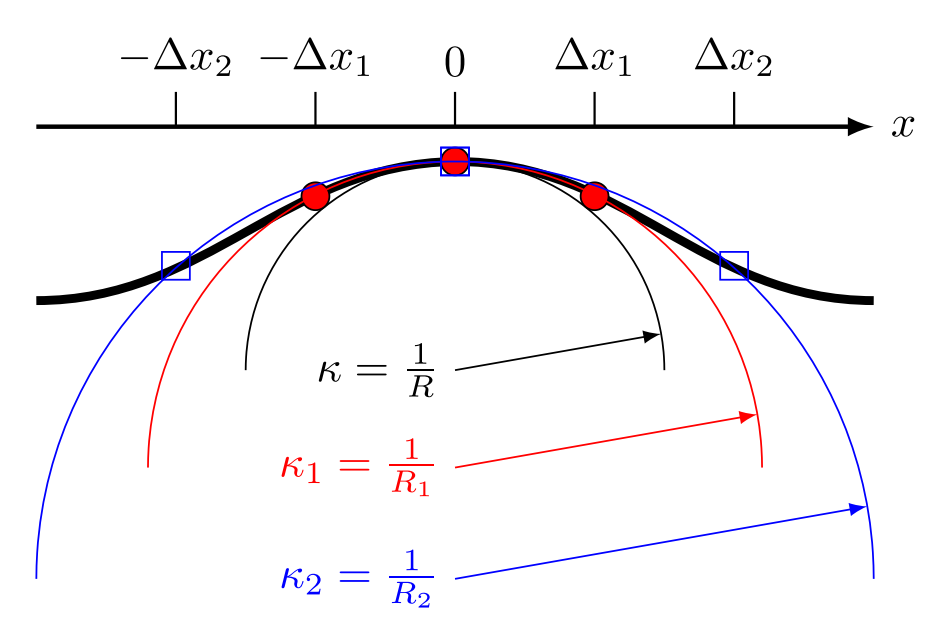
\includegraphics[width=2.5in]{figs/curv}
	\caption{Typical staggered grid, adopted from \cite{TRYG}.}
	\label{fig:curv}
\end{figure}

\noindent \todo{noindent}Accurate simulations of multiphase flows require an accurate estimation of interface curvature. Figure \ref{fig:surf} illustrates this importance by presenting two atomizing jet simulations. These simulations vary only by their Weber number, which is directly proportional to the surface tension term, and thereby, the curvature at the interface. It is clear that the jet seen in Figure \ref{fig:surf}(b) is experiencing far greater breakup than that seen in Figure \ref{fig:surf}(a). The correct representation of reality is highly dependent on the estimation of curvature made by the numerical model. 

 \begin{figure}[htbp]
	\centering
	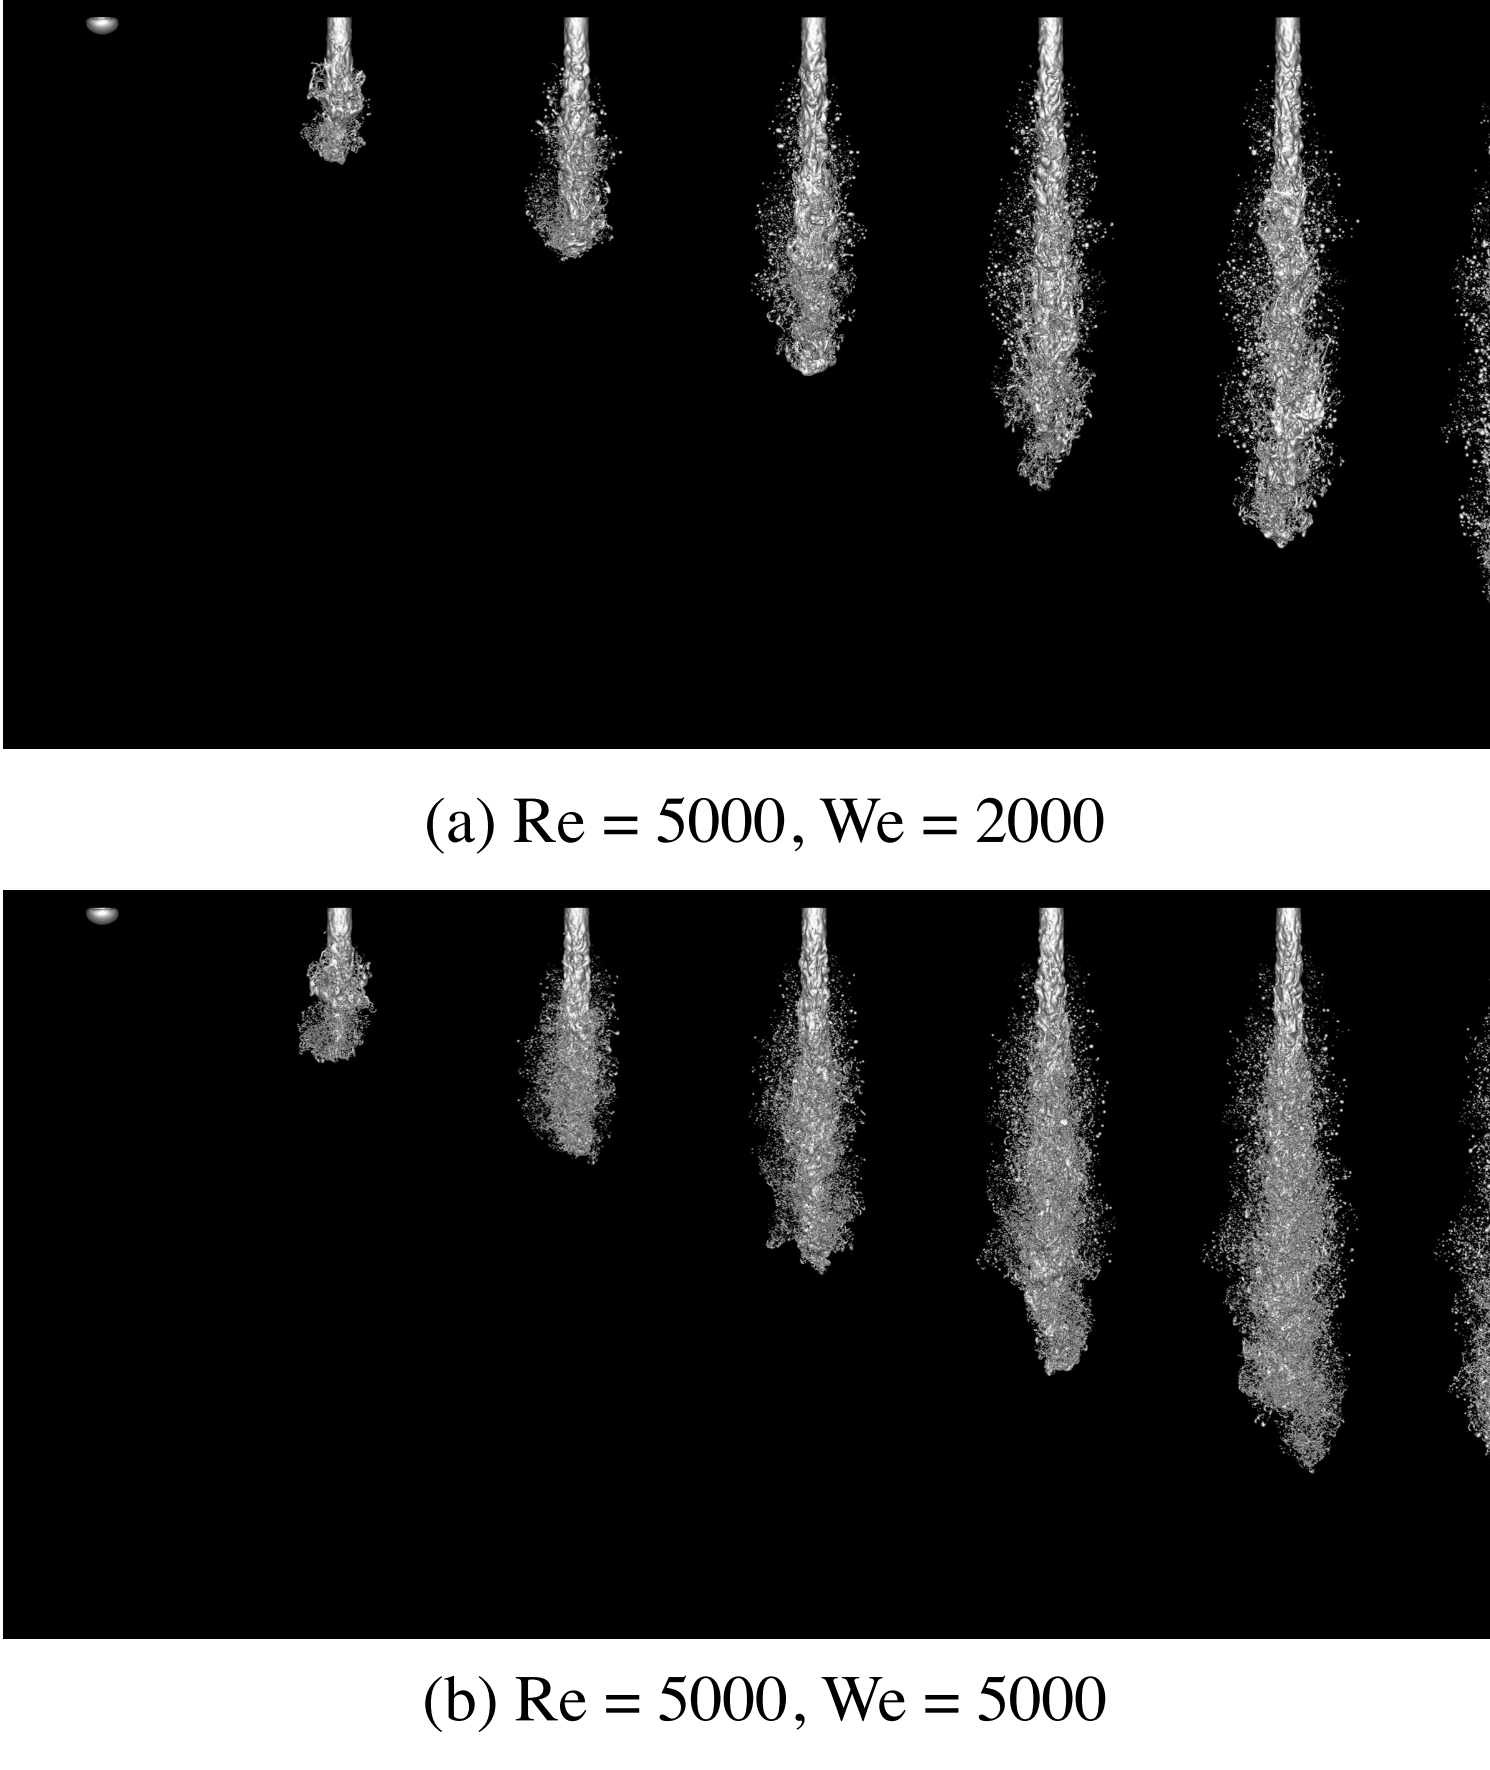
\includegraphics[width=5.0in]{figs/surf}
	\caption{Atomization simulations with varying Weber number, adopted from \cite{Desjardins13}.\hl{figure this spacing out}}
	\label{fig:surf}
\end{figure}

Many techniques exist for calculating values of curvature, some of these include:  \hl{level set methods,  height functions, coupled level set volume of fluid (CLSVOF) methods}\todo{not sure about this list, these seem like mostly interface capturing methods and not ways to compute the curvature}, and others~\cite{1,2,3,4}. The focus of this work specifically, is on modified height function methods.

 \begin{figure}[htbp]
	\centering
	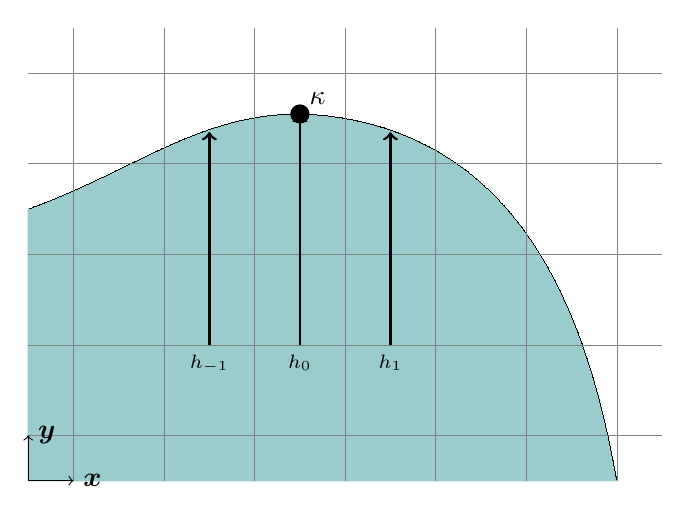
\begin{tikzpicture}[scale=1.15]
		% Mesh
		\draw [step=1.0, help lines] (0.5,0.5) grid (7.5,5.5);
		% Liquid
		\draw [line width=0,fill=lightblue] (0.5,3.5) to[out=20,in=170] (4,4.5) to[out=-10,in=100] (7.0,0.5);
		\draw [lightblue,fill=lightblue] (0.5,3.5) -- (7.0,0.5) -- (0.5,0.5) -- cycle;
		\draw [step=1.0, help lines] (0.5,0.5) grid (7.5,5.5);
		% kappa 1
		\draw [fill] (3.5,4.55) circle [radius=0.1];
		\node [above right] at (3.5,4.55) {$\kappa$};
		\draw [arrows=->,line width=1.0] (2.5,2) -- (2.5,4.35);\node [below] at (2.5,2) {\scriptsize $h_{-1}$};
		\draw [arrows=->,line width=1.0] (3.5,2) -- (3.5,4.55);\node [below] at (3.5,2) {\scriptsize $h_{0}$};
		\draw [arrows=->,line width=1.0] (4.5,2) -- (4.5,4.35);\node [below] at (4.5,2) {\scriptsize $h_{1}$};
		% Triad
		\begin{scope}[shift={(0.5,0.5)}] 
			\draw [arrows=->] (0,0) -- node[pos=1,right] {$\bm{x}$} (0.5,0);
			\draw [arrows=->] (0,0) -- node[pos=1,right] {$\bm{y}$} (0,0.5);
		\end{scope}
	\end{tikzpicture}
	\caption{Traditional height function} 
	\label{fig:hts}
\end{figure}

\noindent Height functions work by integrating volume fractions ($\alpha$) within columns of cells as in \hl{equation}\todo[inline]{choose a consistent way to reference equations and have a tilde} \ref{eqn:hts} to form heights. A similar approach is taken using widths where an interface is more vertical than horizontal.  \todo{add text so the equations flow with the reading.}
 

\begin{equation}
h_{i} = \sum_{i-1}^{i+1} \alpha_{i,j} \Delta y
\label{eqn:hts}
\end{equation}

\noindent Figure \ref{fig:hts} gives an example of heights at a liquid-gas interface. In the simplest execution of a height function, approximation of the curvature ($\kappa$) at the point on the grid is achieved by using a simple finite difference of the heights to approximate first and second derivatives as seen in equations \ref{eqn:1st} and \ref{eqn:2nd} respectively. \todo{Write the equations so they flow}

\begin{equation}
H_{x} = \frac{h_{i-1,j}-h_{i+1,j}}{2 \Delta x}
\label{eqn:1st}
\end{equation}
\begin{equation}
H_{xx} = \frac{h_{i+1,j}-2h_{i,j}+h_{i-1,j}}{ \Delta x^2}
\label{eqn:2nd}
\end{equation}

\noindent Finally, curvature is calculated using:
\begin{equation}
\kappa = \frac{-H_{xx}}{(1+H_{x}^{2})^{\frac{3}{2}}}.
\label{eqn:kap}
\end{equation}

\noindent Clearly the above explanation is relevant for two-dimensional flows. Extension to three-dimensional flows is trivial. \todo{What's Eq. 2.10 in 3D?}

Height functions remain a prevalent method for estimating curvature because of their relative ease of implementation.\todo{and their 2nd order convergence} However, several adjustments to the standard model have been proposed. Adjustments include changing the stencil size over which the heights are gathered~\cite{1}, separating the columns from the computational mesh~\cite{2}, combining heights and widths for approximation~\cite{2}, and applying the approach to level sets~\cite{2}(\hl{this sentence is a paraphrase from Mark's 18 JCP consider revising}).


\subsection{Using Height Functions in Conjunction with Rudman Dual Mesh }

When a dual grid is used, the standard height function method fails to capture the dynamics occurring on the fine grid. Left unmitigated, these dynamics can result in fine grid interfacial perturbations, small discontinuities in interface structures. These perturbations can grow uncontrollably and result in non-physical dynamics materializing in simulations. An example of this uncontrolled growth resulting in non-physical dynamics can be seen in Figure~\ref{bad2}. The focus of this research is to develop an extension of the standard height function to include information from the Rudman dual mesh. This method results in consistent mass and momentum transport while also providing accurate interface transport that avoids non-physical dynamics.


\begin{figure}[htbp]
	\centering
		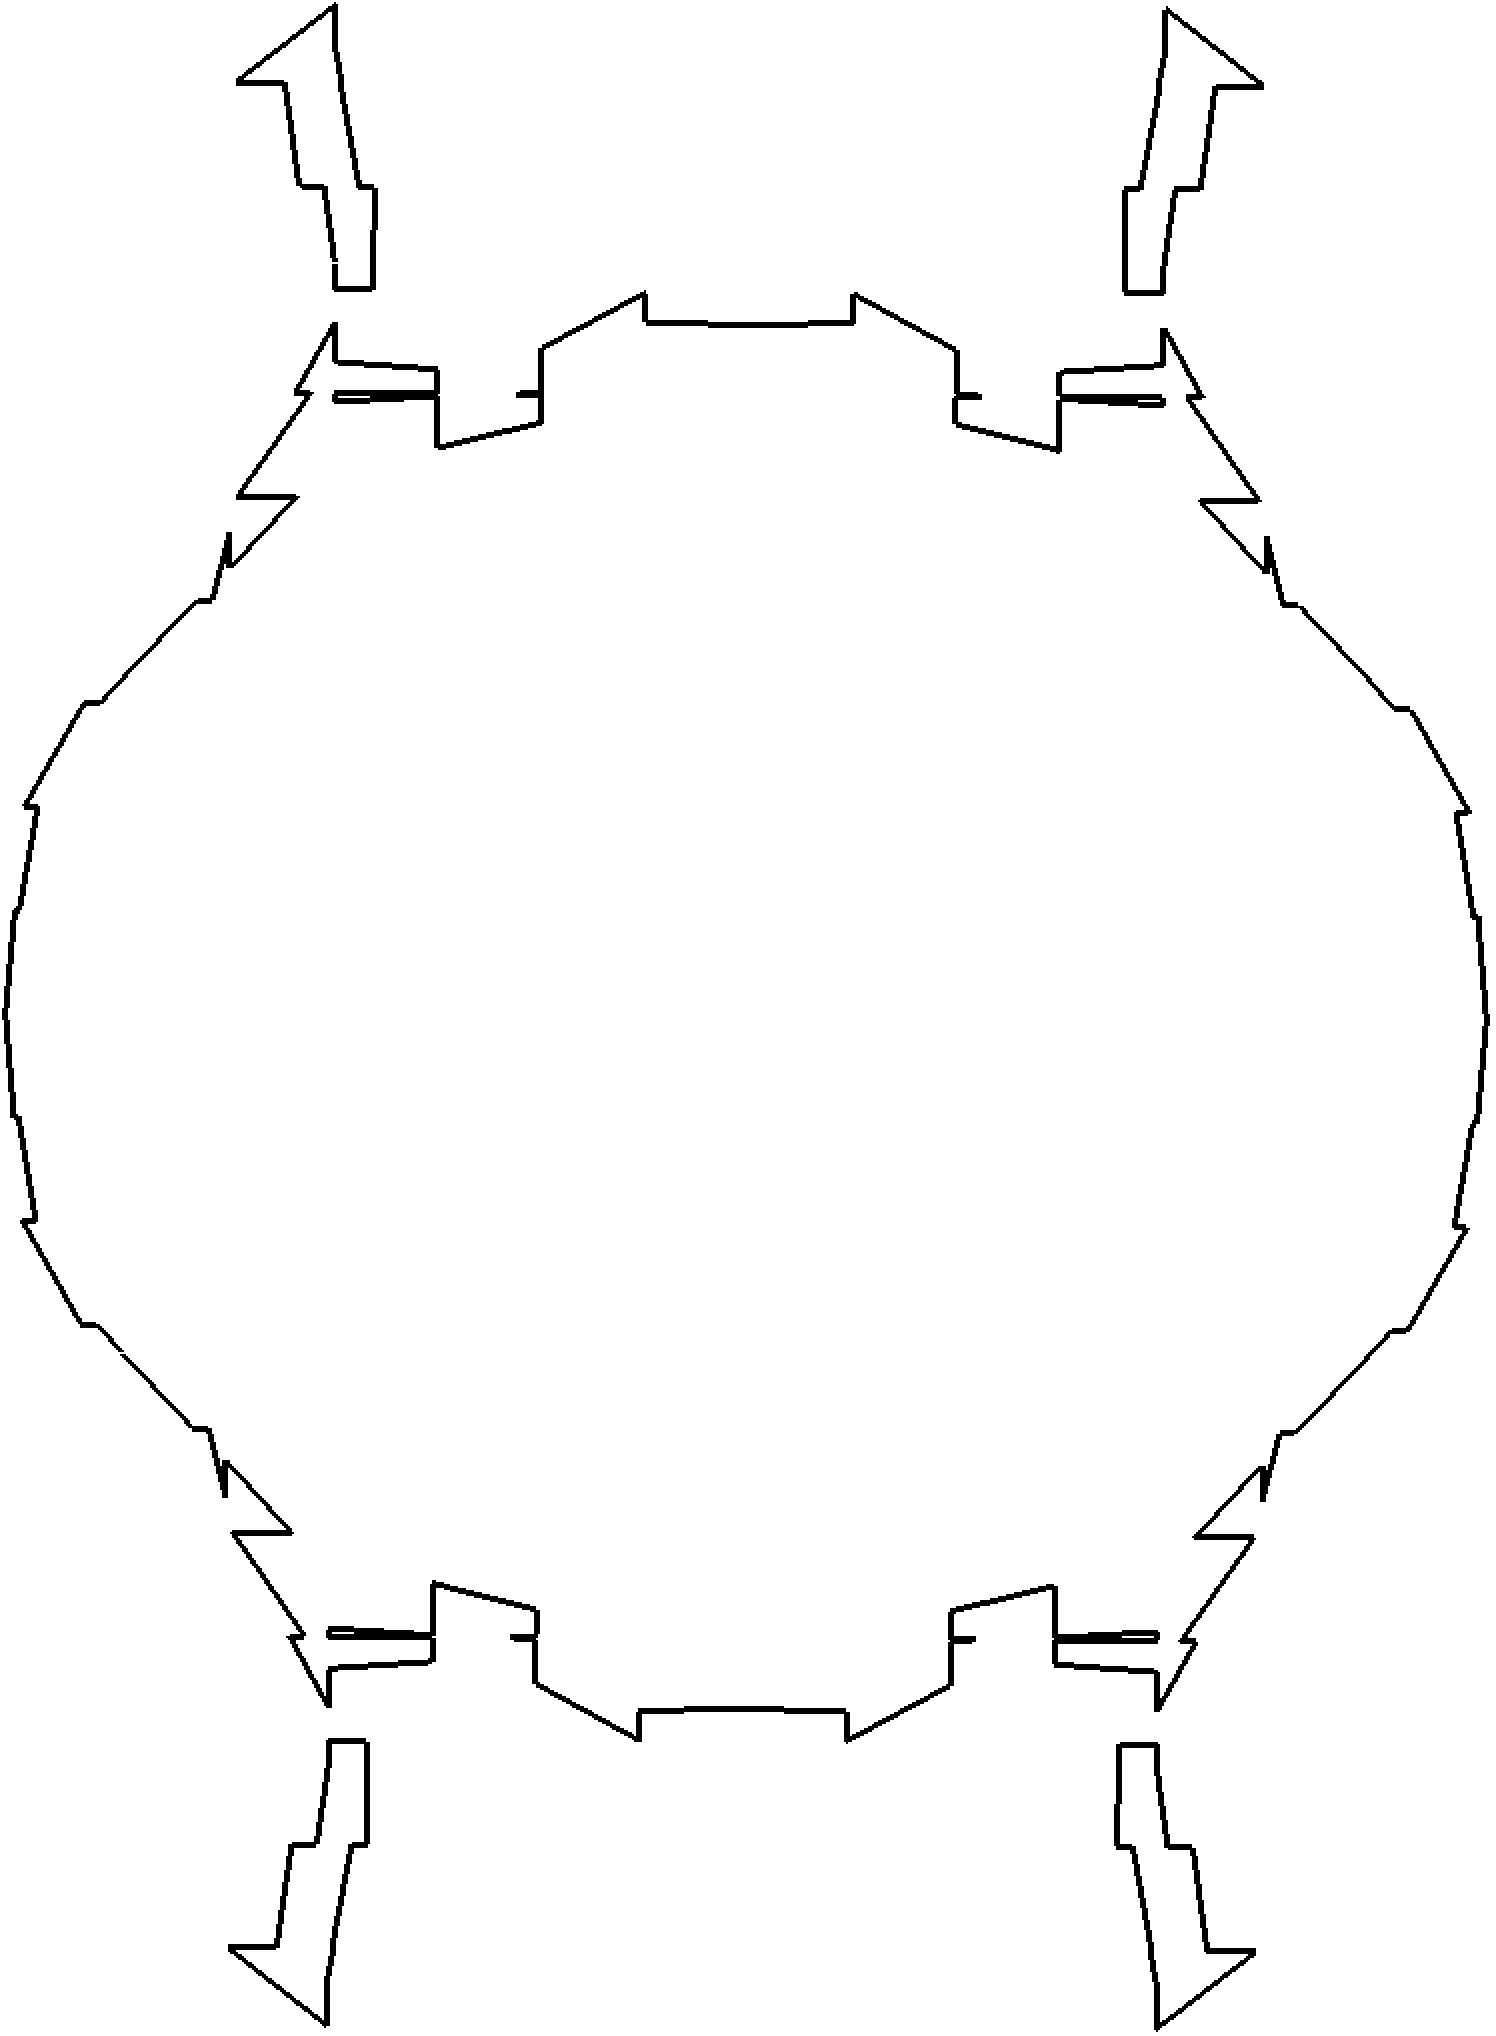
\includegraphics[scale=0.25]{figs/bad.png}
	\caption{Standard method interface breakup.}
	\label{bad2} 
\end{figure} 

\chapter{Methodology} \label{CH:method}
%\textbf{How do you implement your Soln?\\
%Build a Fg HFM\\
%Use fgHFM to compute fgCurv\\
%Use fgCurv to infor cgCurv\\
%Use Curv's to solve RHS eqn\\
%Derive RHS eqn \& ref Herrmann as well as our modifications and $\delta$ approximation\\
%Use RHS to update fgVel\\
%Solve Poisson w/ new fgVel\\
%Fluxes happen somewhere in all of this???\\
%}\\

%This section will focus on the story of how the current model came to be. \\
%Start with the beginning: look on Box for presentations\\
%TIMELINE:\\
%
%
%Feb 2018 - PLIC reconstruction- area of discontinuity $\rightarrow$ velocity to drive back discontinuity\\
%Apr 2018 - velocity correction based on area times some factor $\rightarrow$ gives idea fro subgrid HFM\\
%May 2018- using matlab compute heights and curvature as 1/r \\
%Jun 2018 - Can show 5th order L2 error with mesh refinement (5th order finite difference scheme)\\
%Jul 2018 - ICLASS 2018 Poster - here we've tried several different discretization techniques\\
%Aug 2018 - Reintroduce SG velocity but allow to be influence by curvature rather than area\\
%Oct 2018 - Implement FG HFM but find parasitic wiggles $\rightarrow$ this is start of Herrmann correction and we add in 2nd pressure equation to ensure fine grid divergence free condition (12Oct18 presentation - late october is basically final APS presentation... same with november... thats the state at that point in time )\\
%Jan 2019 - Found discrepancy in Herrmann Eqn \\
%Mar 2019 - delta approximation big parametric study \\
%Apr 2019 - still doing para study \\

%Method development which would include information from the fine grid to reduce interface reconstruction discontinuities. 
%
%Introducing a fine grid velocity 

%With the standard implementation of NGA, VOF is calculated on the fine grid and curvature is computed on the coarse grid. 
%
%
%
%\begin{figure}[htbp]
%	\centering
%	\begin{tikzpicture}[scale=1.5]
%	% PLIC
%	\draw [lightblue,fill=lightblue] (0,0) -- (0,0.7) -- (1,0.7) -- (1,1.3) -- (2,1.3) -- (2,0) -- cycle;	
%	% VOF
%	\node at (0.5,0.5) {0.7};
%	\node at (1.5,0.5) {1};
%	\node at (0.5,1.5) {0};
%	\node at (1.5,1.5) {0.3};
%	%Cell
%	\draw [black, very thick] (0,0) -- (2,0) -- (2,2) -- (0,2) -- (0,0);
%	% Grid
%	\draw [blue, thick, dashed] (1,0) -- (1,2);
%	\draw [blue, thick, dashed] (0,1) -- (2,1);
%	\draw [arrows=->,line width=1.0] (0.5,0.7) -- (0.5,1.3);\node [left] at (0.49,1.1) {\scriptsize $v$};
%	\draw [arrows=->,line width=1.0] (1.7,1.7) -- (1.7,1.3);\node [right] at (1.705,1.5) {\scriptsize $v$};
%	\end{tikzpicture}
%	\caption{Advection of a one-dimensional fluid interface}
%	\label{fig:1Dadvect}
%\end{figure}

\subsection{Oscillating Droplet Test Case}
To further quantify the problem that is occurring, a baseline test case which highlights the shortcomings of current methods is necessary. To this end, an oscillating two-dimensional droplet is used to assess the height function method and the proposed solution methods. This test case was chosen as it is considered a standard benchmark problem for testing the accurate prediction of multiphase flow behavior\cite{Salih2002}. Additionally, for the height function method, the oscillating droplet offers an extensive testing of interface orientations which is important for measuring the robustness of the method. The interface is initialized with an ellipsoid. Surface tension drives the droplet's semi-major axis to fluctuate between alignment with the $x$ and $y$ axes. The period of oscillation $T_{e}$, is a function of surface tension coefficient ($\sigma$), density ($\rho_l$ and $\rho_g$), and equivalent circular radius($R$), and can be computed analytically as~\cite{Rayleigh}
\begin{equation}
T_{e} = 2 \pi \sqrt{\frac{(\rho_{l}+\rho_{g})R^3}{6\sigma}}.
\label{period}
\end{equation}


















































\chapter{Discussion}  
\subsection{Simplified Test Cases}
With each of the schemes previously discussed, the method of evaluation consisted of an explicit curvature calculation of an exact VOF field followed by an oscillating droplet test case. Consistently, the exact curvature estimation was successful and the oscillating droplet problematic. The transition between the test cases began to seem like too great of a jump in complexity to have an intimate understanding of the progression of errors occurring. To gain a deeper understanding of the source of failure, it seemed necessary to have more simplified test cases with which to study the method. To this end, four simplified test cases were developed which we hoped would expose the limitations of the schemes.

\subsubsection{Sine Wave Test Case}
A sinusoidal interface was constructed as seen in Figure~\ref{fig:sine}. The test case was created specifically to test several key aspects of the method. First, by modifying the geometry of the sinusoid its possible to test internal and external face fluxes independently or jointly. Secondly, because the interface is highly symmetric, variation in velocity and curvature values across the domain helps to highlight deficiencies in boundary conditions as well as inter-cell transport schemes. The goal of this test case is for the fine grid scheme to force a collapse of the interface so that a final curvature of zero is achieved.  
 \begin{figure}
 	\centering
 	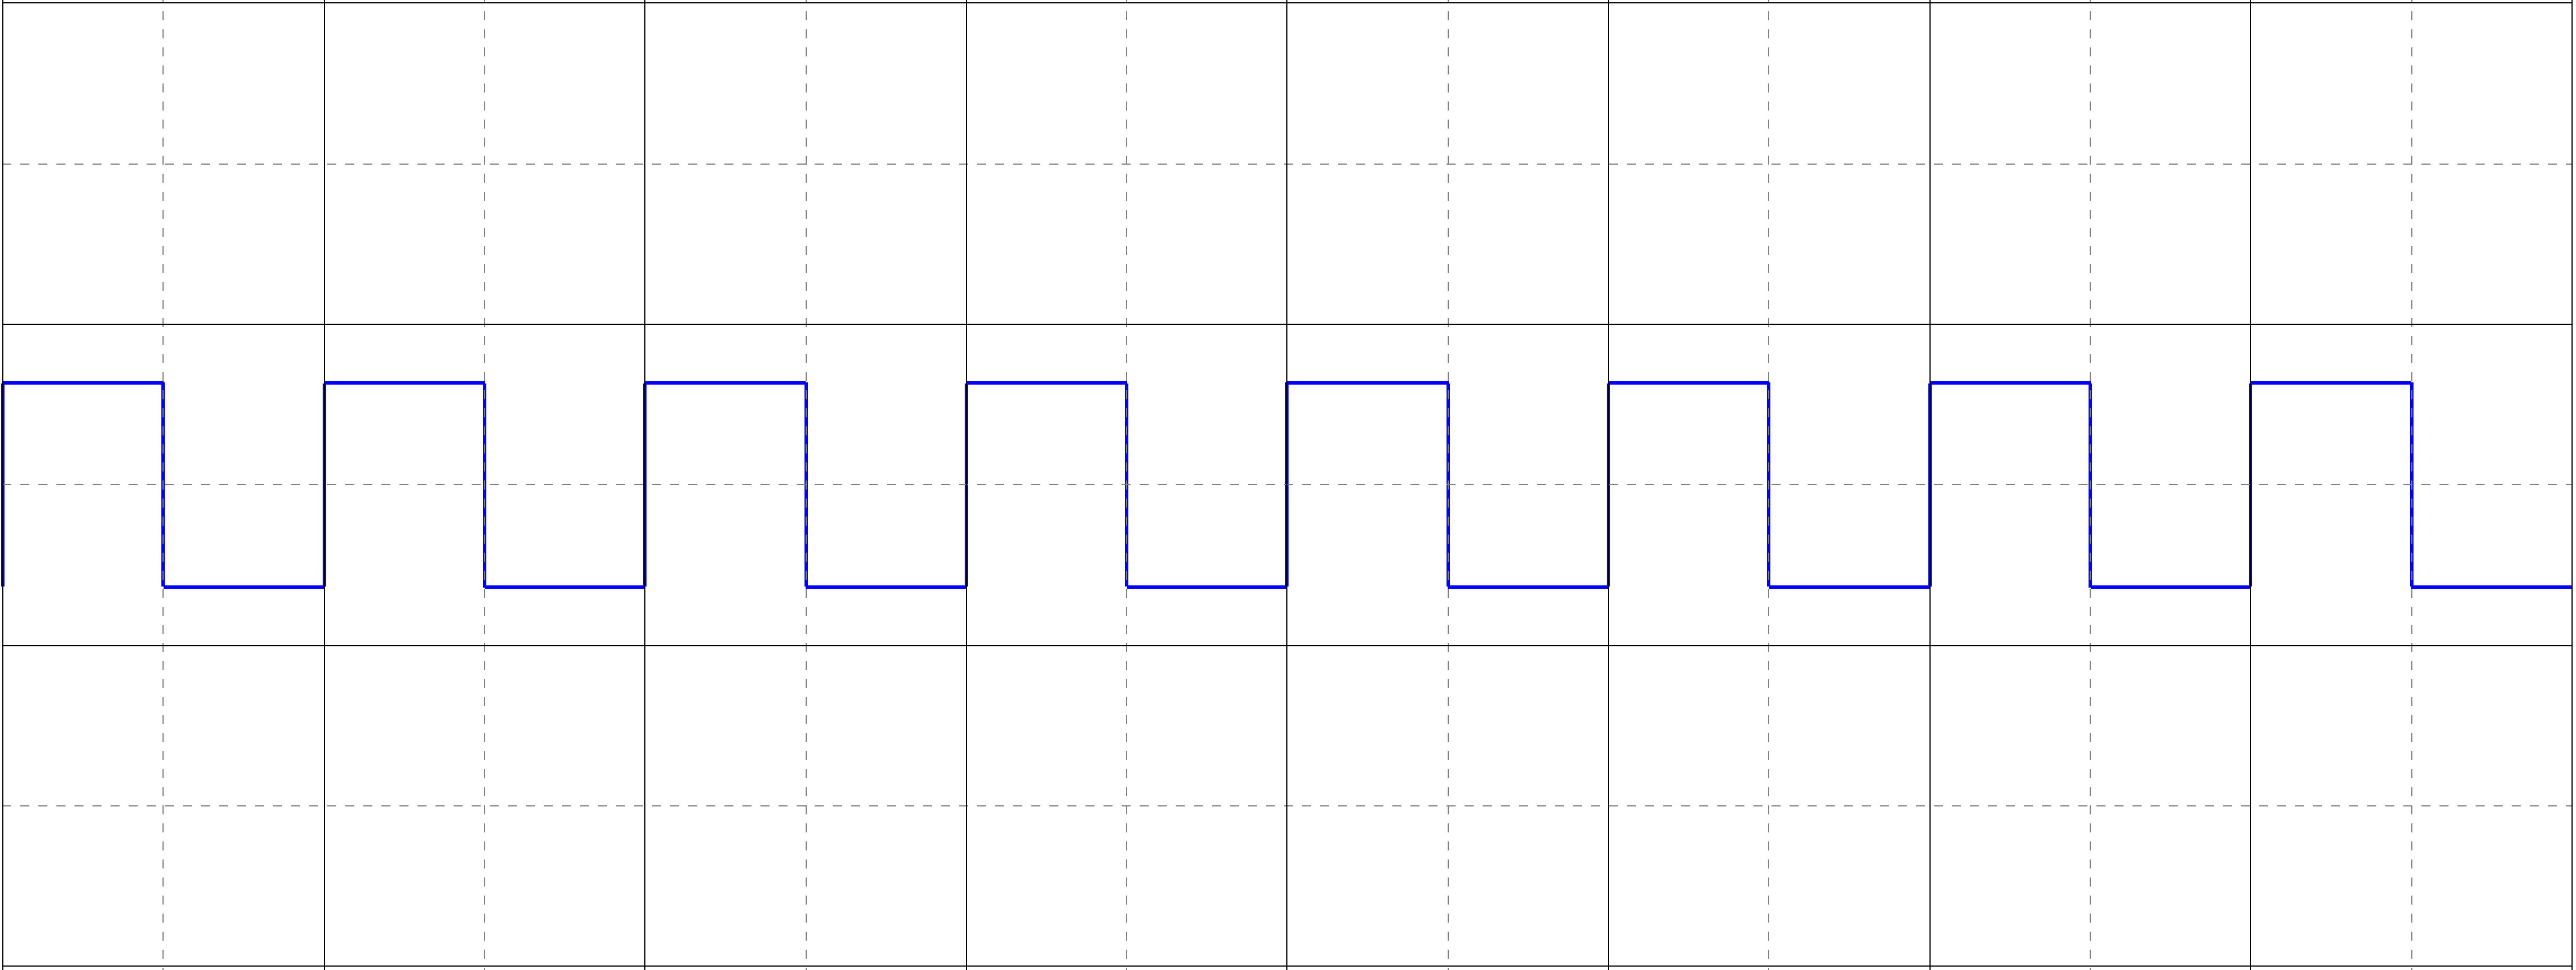
\includegraphics[width=0.5\textwidth]{figs/sine}
 	\caption{fix figure}
 	\label{fig:sine}
 \end{figure}

\subsubsection{Interfacial Protrusion Test Case}
The test cases shown in Figures~\ref{fig:0},~\ref{fig:90}, \&~\ref{fig:45} are all of a simple linear interface at various orientations. At the center of each domain, a protrusion was placed on the interface. The aim of this test case was to recreate specific, isolated, scenarios to see if the fine grid method could accomplish collapsing the interface to a line and obtain a zero curvature across the domain. The protrusion on each interface was built to be approximately one cell width in both height and width. 

\begin{figure}[htbp]
	\centering
	\begin{minipage}{0.3\textwidth}
		\fbox{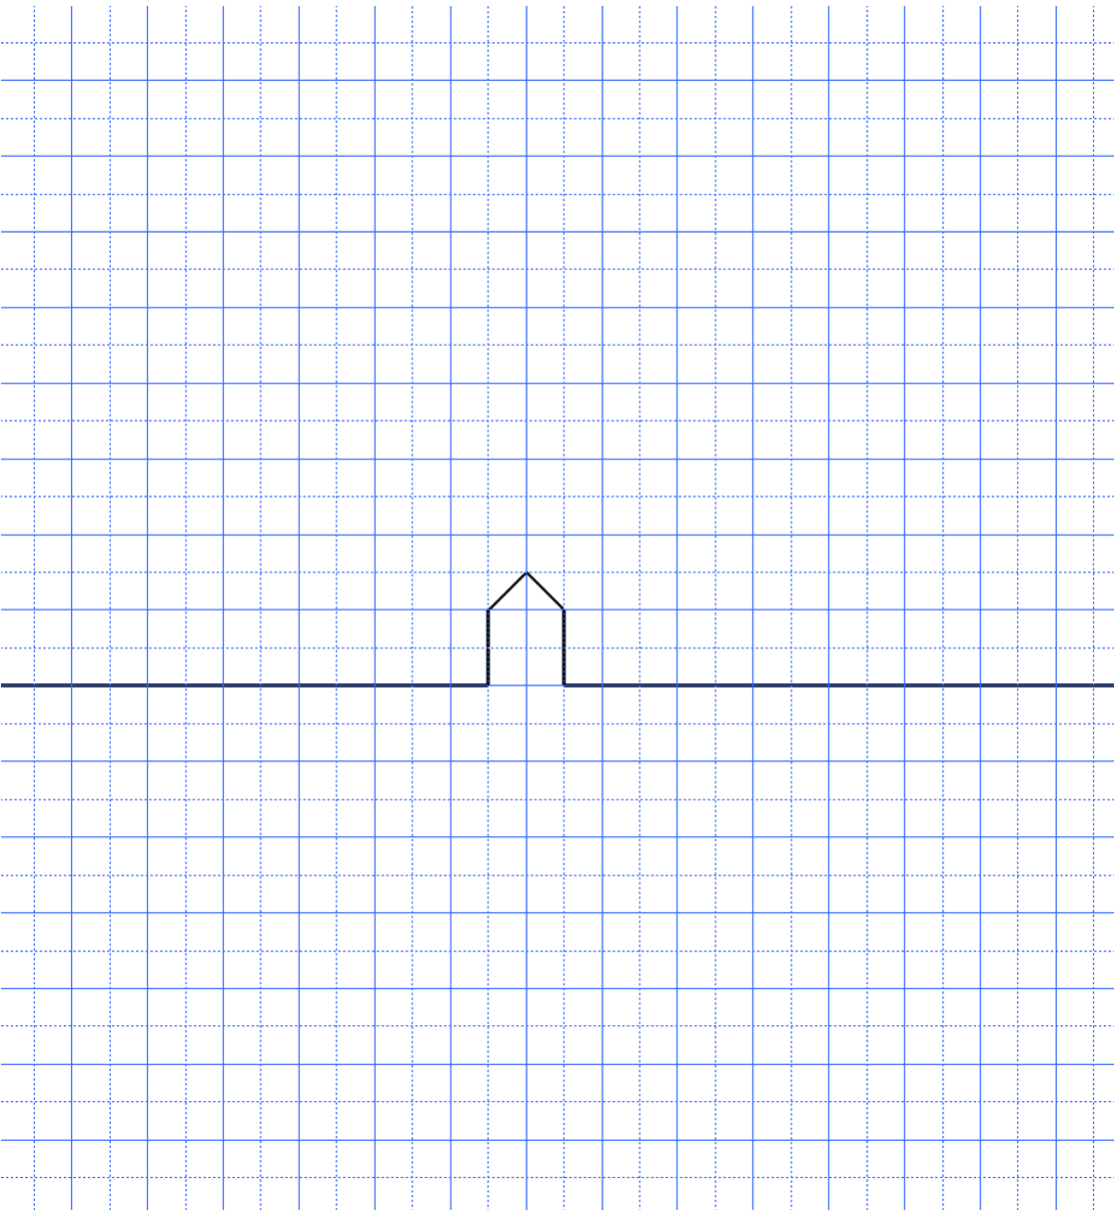
\includegraphics[width=0.95\linewidth]{figs/0}}
		\caption{fix figure}
		\label{fig:0}
	\end{minipage}%
	\begin{minipage}{0.3\textwidth}
		\fbox{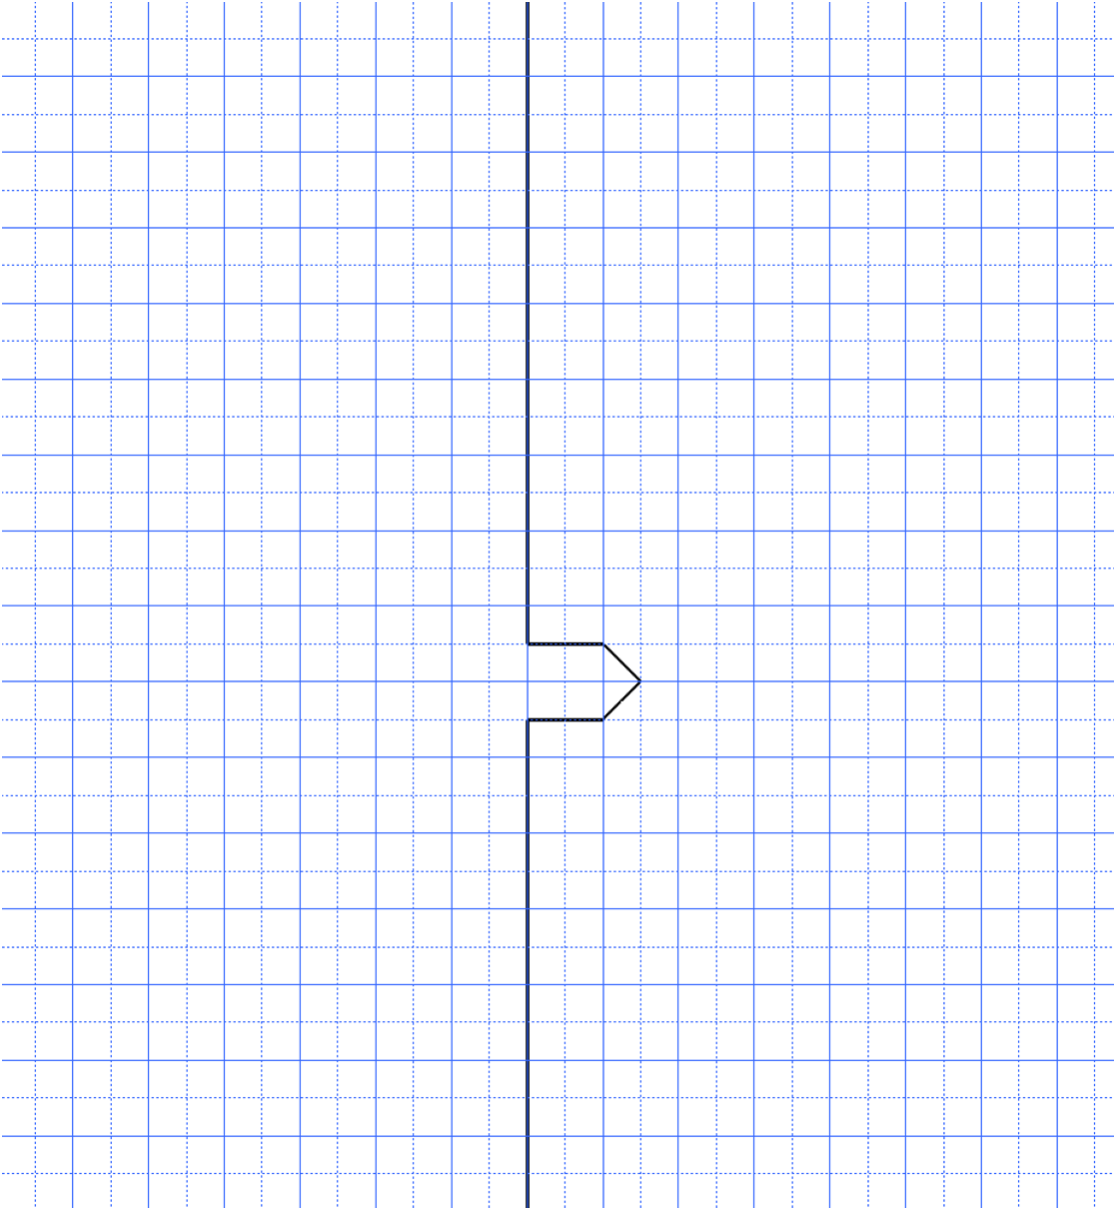
\includegraphics[width=0.95\linewidth]{figs/90}}
		\caption{fix figure}
		\label{fig:90}
	\end{minipage}
	\begin{minipage}{0.3\textwidth}
		\fbox{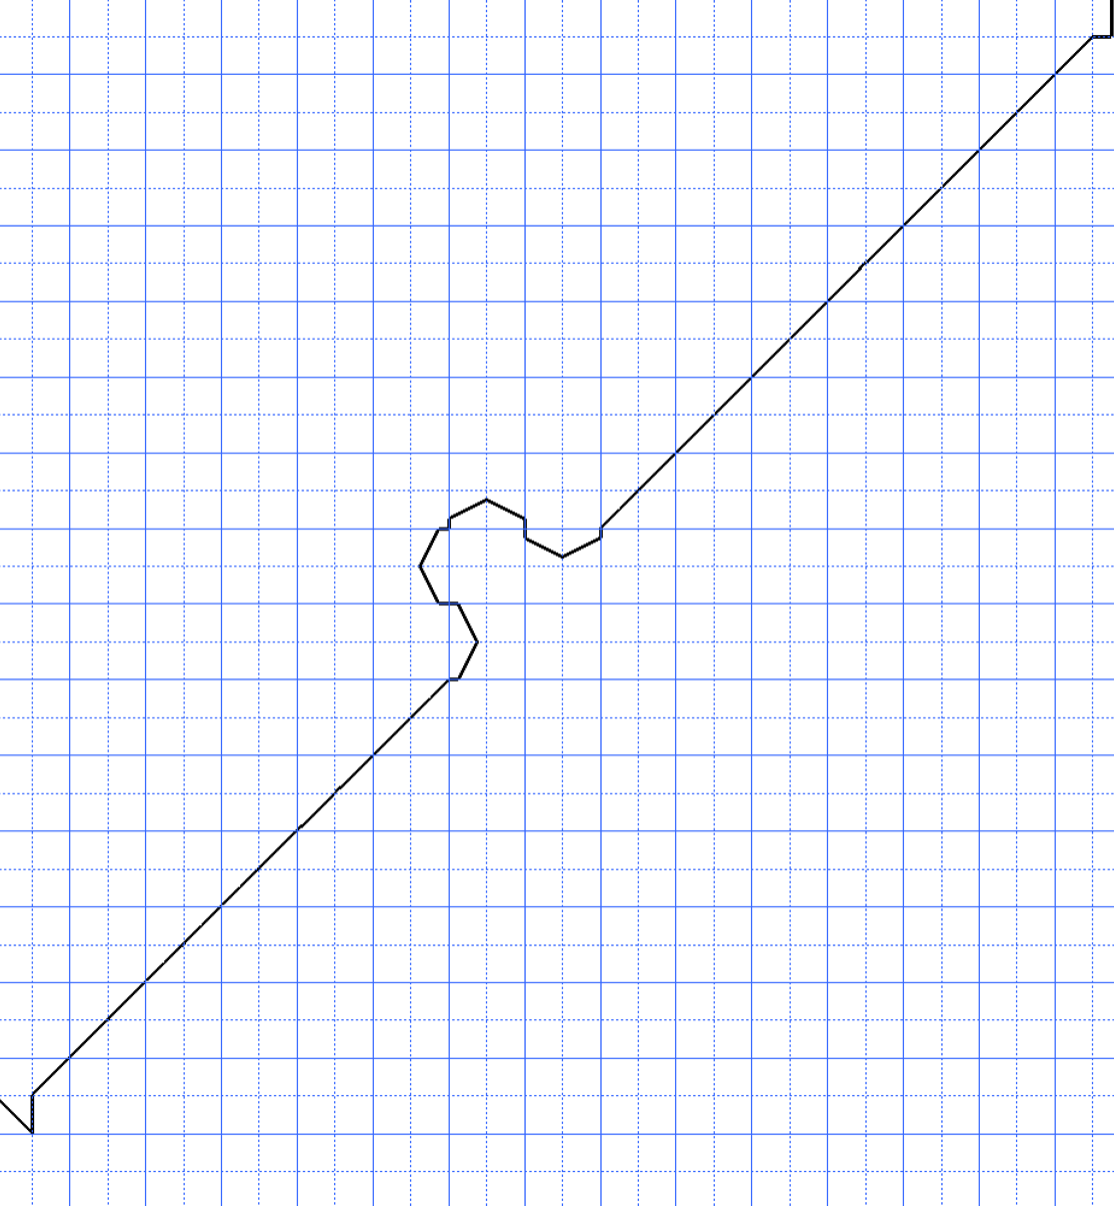
\includegraphics[width=0.95\linewidth]{figs/45}}
		\caption{fix figure}
		\label{fig:45}
	\end{minipage}
\end{figure}

\begin{figure}
	\centering
	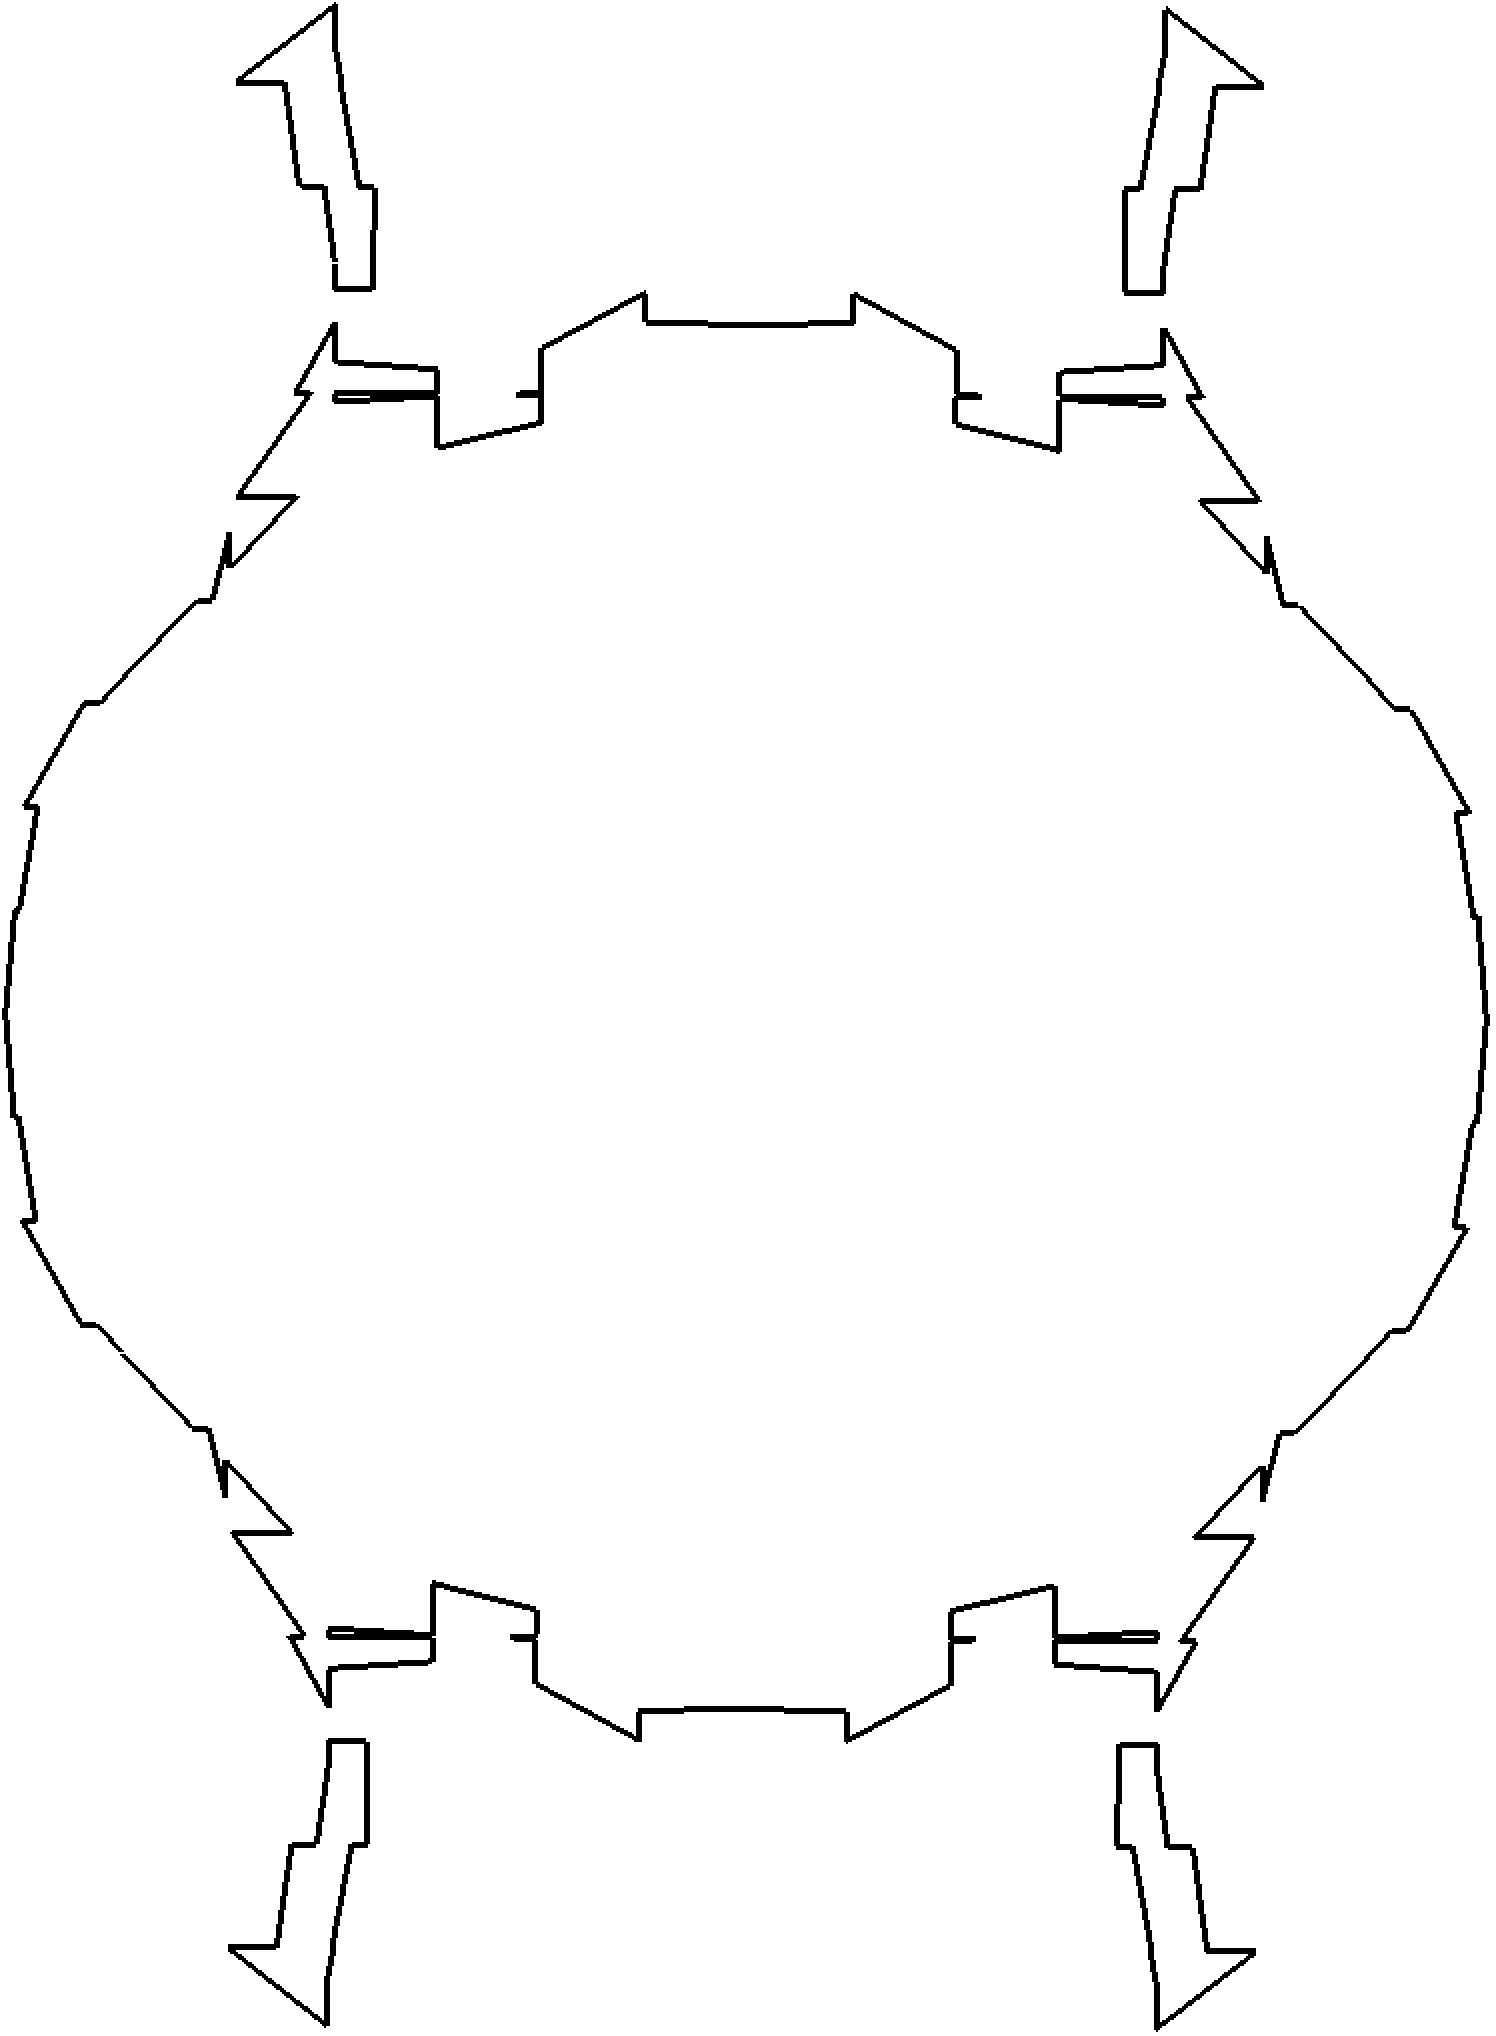
\includegraphics[width=0.5\textwidth]{figs/bad.png}
	\caption{fix figure}
	\label{fig:45s}
\end{figure}
For each of the above test cases, with the exception of the $45^{\circ}$ test case, the method was successful in collapsing the interface to a line. This was an interesting discovery and seemed to coincide with results seen in failing oscillating droplet test cases. During the oscillating droplet test, often nonphysical geometries would begin to appear at each of the quadrant regions of the droplet as shown in Figure~\ref{fig:45s}. This finding exposed a key limitation of the model. Well defined heights are not present in this case and cause problems for the height function method. When heights are not well defined, the approximation of derivatives is not accurate and results in nonphysical geometries.  

At the current state, the fine grid method can successfully predict curvature for a select set of geometries. No successful execution of three dimensional flows have been performed or analyzed. Rigorous investigation of the methods outlined above have left the researchers with several fundamental concerns and drawbacks of this method can be summarized as
\begin{enumerate}
	\item It is clear that this method, in all iterations, requires well defined heights for successful execution. However, achieving well defined heights may require mesh sizes which are unrealistic for direct numerical simulation. While there may possibly be ways to work around this issue, research thus far has focused on performing successful simulations with geometries that provide ideal mesh size ratios. Investigation into more complex schemes should only be attempted after this has been achieved.
	\item Incorporation of fine grid velocities seemed to have a positive impact on success of the system but required several modifications from the originally proposed method. The addition of a second pressure equation makes this method computationally expensive. So much so that simulation run time can increase by $40\%$. This increased expense contradicts original motivation of the investigation. Modification of the height function method was chosen as implementing the method is straightforward and the cost is low compared to more complex methods. To that point, while the fine grid height function is straightforward to implement, fine grid velocity incorporation and the subsequent incorporation of semi-lagrangian fluxes are not. 
	\item While little investigation has been done with three dimensional flow fields, accurate and realistic curvature becomes significantly harder to achieve as fitting is now done using planes instead of lines.
	\item To present, efforts have been considering a simulation which doesn't "blow up" to be a success. However, no efforts have gone into investigating the accuracy of this model. This is vital to understanding the merit of the method. 
\end{enumerate} 

%\begin{figure}
%\begin{tikzpicture}[scale=4.25]
%% Heights
%\draw [black, fill=cyan!20] plot [smooth ] coordinates {(0.25,0.3)(0.75,0.5)(1.25,0.1)(1.75,0.6)(2.25,0.3)(2.75,0.7)} -- (2.75,0) -- (0.25,0) -- cycle;
%\draw [fill] (1.5,0.36) circle [radius=0.05];
%\node [above ] at (1.5,0.45) {$\kappa$};
%\draw [arrows=->,line width=1.0] (0.25,0) -- (0.25,0.3);\node [below] at (0.25,0) {\scriptsize $h_{-3}$};
%\draw [arrows=->,line width=1.0] (0.75,0) -- (0.75,0.5);\node [below] at (0.75,0) {\scriptsize $h_{-2}$};
%\draw [arrows=->,line width=1.0] (1.25,0) -- (1.25,0.1);\node [below] at (1.25,0) {\scriptsize $h_{-1}$};
%\draw [arrows=->,line width=1.0] (1.75,0) -- (1.75,0.6);\node [below] at (1.75,0) {\scriptsize $h_{1}$};
%\draw [arrows=->,line width=1.0] (2.25,0) -- (2.25,0.3);\node [below] at (2.25,0) {\scriptsize $h_{2}$};
%\draw [arrows=->,line width=1.0] (2.75,0) -- (2.75,0.7);\node [below] at (2.75,0) {\scriptsize $h_{3}$};
%\end{tikzpicture}
%\caption{$5^{th}$ Order Fit of Heights}
%\label{fig:5thhts}
%\end{figure}

\subsection{Future Work}
DONT DO IT
%\section{Outline}
%\begin{Verbatim}[tabsize=4]
%	-We currently have a method that "kind of" works
%		*2D has been majority of testing
%	-We've learned that well defined heights are essential at all scales
%	-Drawbacks of this method:
%		*Well definied hts req mesh sizes that may be unrealistic for 
%		 multphase DNS sims
%		*Additional pressure eqn makes this method incredibly expensive 
%			-this is counter to our original motivation of cheap and easy
%			-To be fair, we're using Gauss Sidel and this leaves room 
%			 for improvement
%		*Moving to 3D becomes more complex as hts are now built with
%		 planes instead of PLIC's
%			-Further investigation needed to determine limitations
%		*Up until now oour metric of success has been "does the sim blow up?"
%			-if not we move on... but, no analysis has been done to test how 
%			  accurate the scheme is
%\end{Verbatim}
% Add additional chapters here

	% REFERENCES
\bibliographystyle{abbrv} % Use a style you and your adviser like
\bibliography{mybib.bib} % Bibliography.  Add your .bib file(s) here


% APPENDIX
% If you have an appendix use either the option appendsingle (1 appendix) or appendmultiple (>1 appendix) in your document class
% If you do not have an appendix comment out below and remove the appendsingle/multiple option from the document class
\appendix
\chapter{Example Code}\label{appendixa}
\textbf{ Include relevant codes $\rightarrow$ multiphase finegrid.f90, multiphase curv.f90, multiphase fluxes.f90 etc }

\chapter{Integral Height Function Coefficient Code}\label{appendixb}
The following code was written in Matlab to find finite difference coefficients for the integral $5^{th}$ order  height function method.
\begin{verbatim}
%function [ hx,hxx ] = weights
% Compute weights for 5th order height function method
clear; clc

syms x z xik zik dx_ dz

% Order of expansion
M=5; N=0;

% Taylor series incluing upto max(M,N) order terms
h=sym(zeros(M+1,N+1));
for n=0:N
for m=0:M
h(m+1,n+1)=(x-xik)^m*(z-zik)^n/(factorial(m)*factorial(n));
end
end

% Allocate Matrices
Z=sym(zeros((M+1)*(N+1),(M+1)*(N+1)));

B=sym(eye  ((M+1)*(N+1),(M+1)*(N+1)));

% Loop over cells in stencil
c=0;
for kp=0;%-3:2
for ip=-3:2
c=c+1; % Column number
%fprintf('%i/6 \n',c)
% Integrate h over this cell to form height
H=int(h,x,xik+(ip)*dx_,xik+(ip+1)*dx_)/(dx_);
% Get coefficents from F
Z(:,c)=H(:);
end
end

% Constrained least squares that enforces 2nd-order 
% finite difference opperators and pushes magnitude
%%Z(6,

% Solve for A's (in a vector)
Av=Z\B;

%%   Weights for needed derivatives    %
% ------------------------------------ %
dx_=1;
c=0;
for n=0;%:N
for m=0:M
c=c+1;
if     m==1 && n==0;  hx =eval(reshape(Av(:,c),6,1)); % h_x
elseif m==0 && n==1;  hz =eval(reshape(Av(:,c),5,5)); % h_z
elseif m==2 && n==0;  hxx=eval(reshape(Av(:,c),6,1)); % h_xx
elseif m==0 && n==2;  hzz=eval(reshape(Av(:,c),5,5)); % h_zz
elseif m==1 && n==1;  hxz=eval(reshape(Av(:,c),5,5)); % h_xz
end
end
end
% Test accuracy
figure(1); clf(1)
syms x z
% Function
f=x^5+2*x*cos(x);
% Location to compute derivative
xo=1;
zo=1;

% Compute integral of f for construction of heights
syms z1 z2 x1 x2
intf=matlabFunction(int(int(f,z,z1,z2),x,x1,x2),'Vars',[x1,x2,z1,z2]);

% Loop over derivatives to test
c=0;
for n=0:N % d/dy^n
for m=0:M % d/dx^m
c=c+1;
% Get correct A's for this derivative
A=reshape(Av(:,c),6,1);

% Grid size to compute heights on
dxs=[1,1/2,1/4,1/8,1/16,1/32,1/64];
error=zeros(1,length(dxs));
for ndx=1:length(dxs);
dx=dxs(ndx);
dz=1; %dxs(ndx);
exact=subs(diff(diff(f,z,n),x,m),[x,z],[xo,zo]);
% Compute heights
ht=zeros(6,1);
for j=0;%-2:2
for i=-3:2
ht(i+4,j+1)=intf(xo+(i)*dx,xo+(i+1)*dx,zo+(j-1/2)*dz,zo+(j+1/2)*dz)/(dx*dz);
end
end

% Perform sum(A*heights) (Evaluates A with this dx/dy)
dx_=dx;
computed=sum(sum(eval(A).*ht));

% Analysis
error(ndx)=abs(exact-computed);
%fprintf('Exact=%5.5f, Computed=%5.5f, Error=%5.5e\n',exact,computed,error(ndx))
end
%         subplot(N+1,M+1,c)
%         loglog(dxs,error,'-o')
%         hold on
%         loglog(dxs,dxs.^5)
%         title(['d/dx^',num2str(m),' d/dy^',num2str(n)])
%         drawnow 
if c==2 || c ==3 
h=figure(c); clf(c)  
plot(N+1,M+1)
loglog(dxs,error,'-.','LineWidth',3)
hold on
loglog(dxs,dxs.^5,'LineWidth',3)
title(['d/dx^',num2str(m),' d/dy^',num2str(n)],'interpreter','latex','fontsize',16)
legend('5th Order Method','5th Order', 'Location', 'NorthWest')
set(gca, 'Color', 'none','Fontsize',16);
drawnow 
basefile = 'figs';
saveas(h,fullfile(basefile,['WeightsDer',num2str(c),'.png']));
end
end
end

%% Convert to Fortran notation (Removing
% hx = [-1/15; -1/9; -1/3;  1/3; 1/9; 1/15];
% hx = [-1/8; -1/8;    0;    0; 1/8; 1/8];
% hxx= [ 1/8;  1/8; -1/4; -1/4; 1/8; 1/8];
dhs={'hx','hxx'};
dx_=1;
dz_=1;
for n=1:length(dhs)
dh=eval(dhs{n});
for kp=0;%-2:2
%         for ip=-3:2
%            strs{ip+4}=eval(dh(ip+4,kp+1));
%         end
fprintf('data dhd%s(:,%+i) / %+5.15e_WP, %+5.15e_WP, %+5.15e_WP, %+5.15e_WP, %+5.15e_WP, %+5.15e_WP / \n',dhs{n}(2:end),kp,dh);
end
end
%end

\end{verbatim}

\end{document}
% do not put anything after this

